\documentclass[german,bachelor]{webisthesis}
%\documentclass[english,master]{webisthesis}
% When you change the language, pdflatex may halt on recompilation.
% Just hit enter to continue and recompile again. This should fix it.

%
% Values
% ------
\ThesisSetTitle{Bauhausboards - Interactive Door Signs for the Office}
\ThesisSetKeywords{These, Are, My keywords} % only for PDF meta attributes

\ThesisSetAuthor{Andr\'{e} Karge}
\ThesisSetStudentNumber{110033}
\ThesisSetDateOfBirth{1}{8}{1990}
\ThesisSetPlaceOfBirth{Jena}

\ThesisSetSupervisors{Junior-Prof. Dr. Florian Echtler,Prof.\ Dr.\ Unknown Yet}

\ThesisSetSubmissionDate{26}{11}{2015}

%
% Suggested Packages
% ------------------
\usepackage[sort&compress]{natbib}
%   Allows citing in different ways (e.g., only the authors if you use the
%   citation again within a short time).
%
\usepackage{booktabs}
%    For tables ``looking the right way''.
%
%\usepackage{tabularx}
%    Enables tables with columns that automatically fill the page width.
%
%\usepackage[ruled,algochapter]{algorithm2e}
%    A package for pseudo code algorithms.
%
%\usepackage{amsmath}
%    For tabular-style formatting of mathematical environments.
%

% Create links in the pdf document
% Hyperref has some incompatibilities with other packages
% Some other packages must be loaded before, some after hyperref
% Additional options to the hyperref package can be provided in the braces []
\usehyperref[backref] % This will add back references in the bibliography

\begin{document}
\begin{frontmatter}
  \begin{abstract}
    Diese Bachelorarbeit befasst sich mit dem Entwurf, der Umsetzung und dem Test von personalisierten
digitalen Türschildern zur Präsentation und Kommunikation im Bürobereich, genannt
%mit dem Namen
Bauhausboards.\\\\
Ziel ist es, eine Anwendung zu erstellen, mit der Nutzer in Büros individuelle Daten präsentieren können.\\
In den meisten Büros sind dazu Pinnwände oder Whiteboards angebracht. Diese bieten jedoch nicht die Möglichkeit den Inhalt anzupassen oder hinterlassene Nachrichten zu lesen, wenn man nicht persönlich vor Ort ist.\\
Zu diesem Zweck wurde eine Web-Applikation entworfen, welche auf, neben Büroeingängen aufgehangenen Tablet-PCs angezeigt wird und mit denen Nutzer im Büro, sowie vorbeigehende Nutzer interagieren können.
Diese muss leicht bedienbar und zusätzlich von Desktop-PCs oder Smartphones benutzbar sein.\\
Nutzer in den Büros können vom Büro aus oder von unterwegs individuelle Daten präsentieren, sowie ihren aktuellen Status setzen.\\
Besucher können dadurch vor Ort über aktuelle Arbeiten, kurzfristige Abwesenheit oder andere interessante Informationen in Kenntnis gesetzt werden. Zudem haben sie die Möglichkeit bestimmten Nutzern des Raumes Nachrichten zu schreiben.\\
Die Applikation wird, um Interaktion und Benutzbarkeit zu erproben, einem Testlauf unterzogen und das Ergebnis anschließend ausgewertet.
  \end{abstract}

  \tableofcontents

  %\chapter*{Acknowledgements} % optional
  %I thank the authors of the webisthesis template for their excellent work!

  %\listoffigures % optional

  %\listoftables % optional

  %\listofalgorithms % optional
  %    requires package algorithm2e

  % optional: list of symbols/notation (e.g., using the nomencl package)
\end{frontmatter}
\chapter{Einleitung}\label{Einleitung}
In Forschungseinrichtungen und in Unternehmen arbeiten viele Menschen mit unterschiedlichen Aufgaben und Tätigkeiten.
Die meisten wissen jedoch nichts darüber was andere Mitarbeiter machen, wenn sie nicht direkt mit ihnen zusammen arbeiten.
Manche Mitarbeiter wollen ihre Kollegen oder Gäste über ihre aktuelle Arbeit, wichtige Termine oder kommende Veranstaltungen informieren.
Andere wollen gern den Inhalt ihrer letzten wissenschaftlichen Ausarbeitung, die Ergebnisse der letzten Konferenz, Noten einer bestimmten Prüfung oder einfach nur private Daten präsentieren.
Um diese Informationen zur Verfügung zu stellen werden in den meisten Büros Pinnwände oder Whiteboards neben den Türen aufgehangen \abb{img:pinnwand}. Um kurze Nachrichten zu hinterlassen kleben Leute Post-Its an ihre Tür oder hängen Do-Not-Disturb Schilder an den Türknauf, wenn sie nicht gestört werden wollen.
\\
\begin{figure}[h!]
  \centering
  %\captionsetup{justification=centering}
    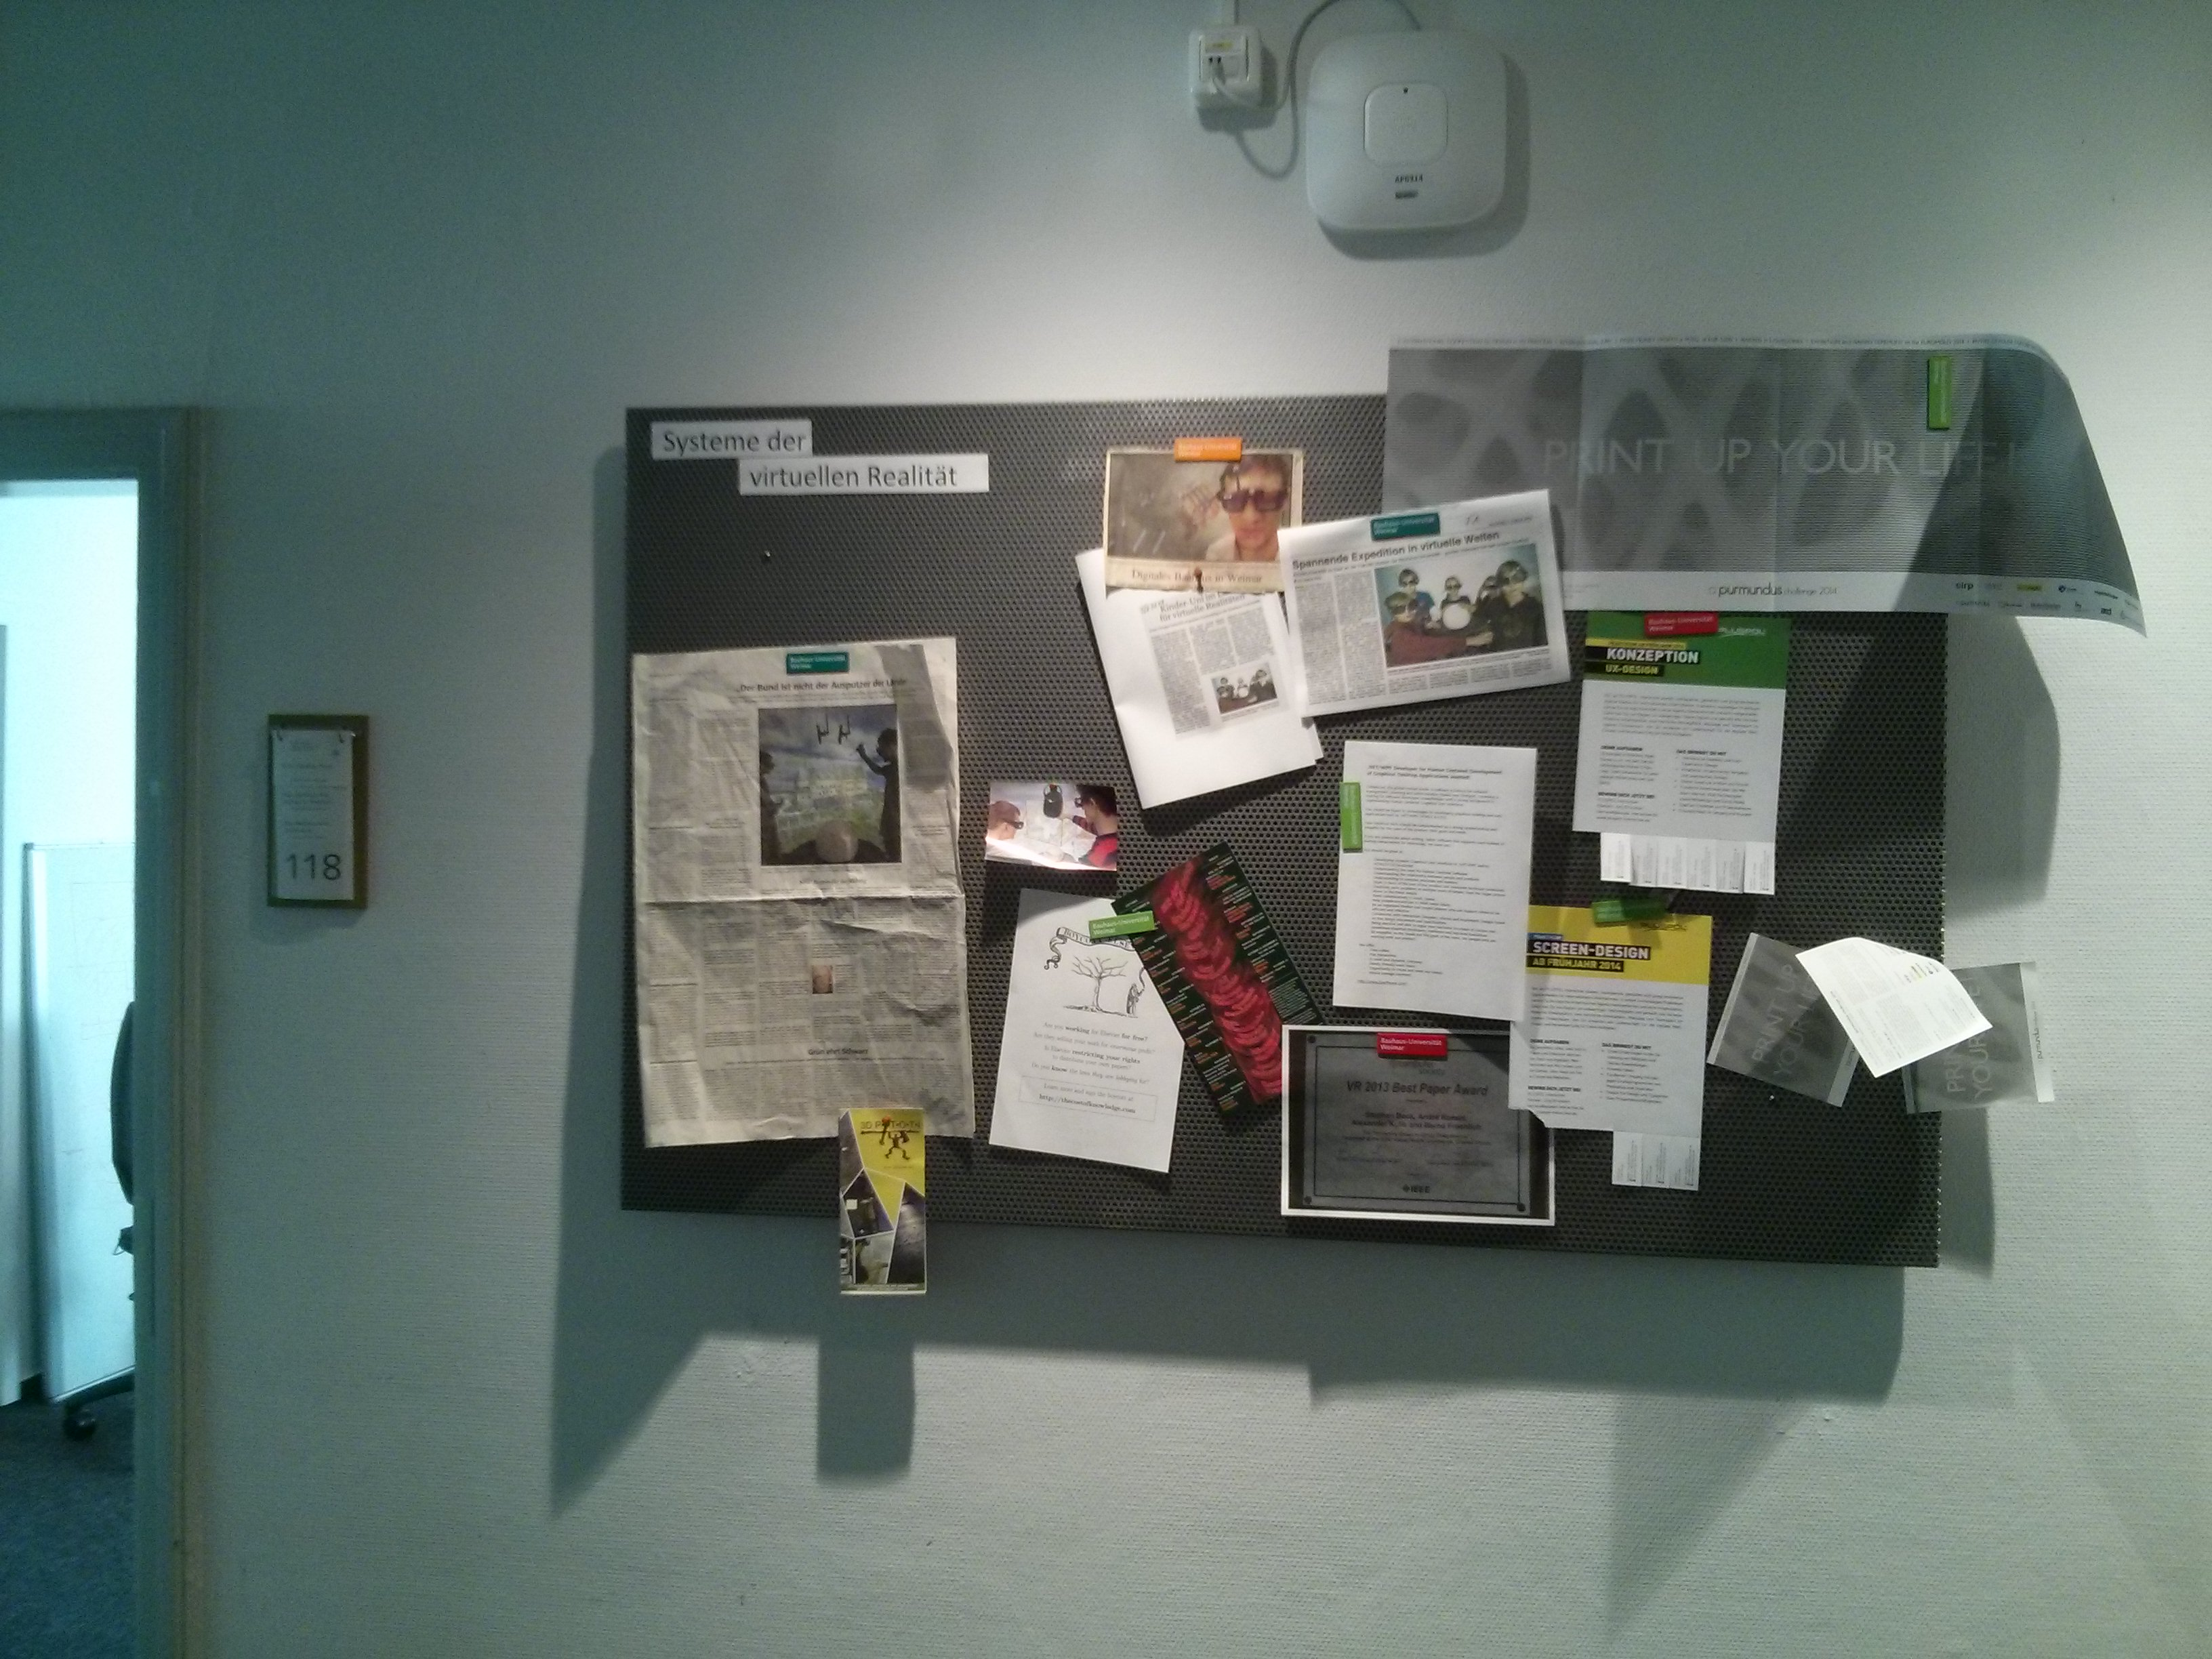
\includegraphics[width=0.6\textwidth]{./img/pinnwand.jpg}
  \caption{Typische Pinnwand der Medienfakultät der BUW}
  \label{img:pinnwand}
\end{figure}
Aktuell müssen die Personen des Raumes solche Informationen direkt an die Wand schreiben oder ausdrucken und danach dort aufhängen.
Wenn man aber nicht persönlich vor Ort ist, kann man die Daten an der eigenen Pinnwand nicht selber anpassen.
Es kann zu Problemen kommen, wenn man einen Termin vereinbart hat und sich dann verspätet, wenn man krank geworden ist und deswegen den ganzen Tag nicht anzutreffen ist oder auf einer Reise ist und andere am Arbeitsplatz direkt daran teilhaben lassen will.
\\
Pinnwände und Whiteboards bieten zudem auch nicht die Möglichkeit digitale Informationen, wie Videos, Animated-Gifs oder die neuesten Twittermeldungen anzuzeigen.
\\
Eine Lösung für diese Probleme ist die Anbringung eines digitalen Türschildes, mit dem Nutzer direkt oder aus der Ferne interagieren können.
\\
\\
Zu Beginn galt es zu klären, welchen Weg ich mit dieser Arbeit einnehmen sollte. Zum einen konnte ich ein bereits vorhandenes Projekt hernehmen, anpassen und verbessern oder ein eigenes System von Grund auf selbst entwerfen und umsetzen.
Deshalb führte ich ein Experiment mit dem NetBoards System\cite{wood:2014,netboards:website} durch um herauszufinden, ob dies ein geeignetes System für die Verwendung an der Medienfakultät der BUW wäre. Zudem ging es darum die Bedürfnisse und das Verhalten der Benutzer im Bezug zu interaktiven Türschildern zu ermitteln.
\\
Nach der Durchführung des Experimentes stellte sich heraus, dass das NetBoards System nicht der richtige Ansatz für die Umgebung war. Deswegen entschied ich mich dazu ein eigenes System zu entwerfen.
\\
Die Entwicklung meines Systems teilte sich in drei Abschnitte: Planungsphase, Implementationsphase und Studienphase.
Die Planungsphase diente dazu die Systemumgebung und den Aufbau der Applikation zu definieren.
Darunter fielen die Wahl des Anwendungstyps und der Programmiersprache, sowie der Entwurf einer Datenbank und des Benutzerinterfaces.
\\
In der Implementationsphase befasste ich mich damit, die geplanten Ideen in ein lauffähiges Programm umzusetzen.
\\
Das Programm musste nach seiner Fertigstellung getestet werden. Deswegen habe ich in der letzten Phase eine Studie geplant und durchgeführt. Dafür habe ich in der Medienfakultät der BUW vor bestimmten Büros Tablets aufgehangen, die Interaktionen damit archiviert und im Anschluss die Büro-Insassen befragt. Die Ergebnisse der Befragung wurden ausgewertet und fließen in die nächste Version des Programms.
\chapter{Vorstudie}\label{Vorstudie}
%%%%%%%%%%%%%%%%%%%%%%%%%%%%%%%%%%%%%%%%%%%%%%%%%%%%%%%%%%%%%%%%%%%%%%%%%%%%%%%%
%Florian-Note:
%Hier würde ich dann als Überleitung erst mal drauf eingehen, wie die existierenden Arbeiten das Design der Vorstudie beeinflusst haben, also z.T. das, was Du jetzt grade in Kapitel 4 schreibst..
%%%%%%%%%%%%%%%%%%%%%%%%%%%%%%%%%%%%%%%%%%%%%%%%%%%%%%%%%%%%%%%%%%%%%%%%%%%%%%%%
%vorüberlegung mit - altes projekt aufsetzen, neues projekt machen?
%\todotext{Übergang - wie haben die Arbeiten das Design der Vorstudie beeinflusst?}\\
%\todotext{ist teilweise schon im kap.4}\\
%Anforderungsanalyse
Zu Beginn war es wichtig eine Anforderungsanalyse durchzuführen. Deshalb galt es, herauszufinden, in welchem Rahmen sich diese Arbeit bewegen sollte. Es bestanden die Optionen, ein fertiggestelltes Projekt anzupassen und zu verbessern oder ein vollkommen eigenes System zu entwickeln.\\
Um zu erproben, wie ein bereits fertiges System funktioniert und wie es von Studenten und Mitarbeitern der Medienfakultät der BUW aufgenommen werden würde, habe ich die Entscheidung getroffen vorerst ein bereits vorhandenes Projekt herzunehmen und in der Praxis zu testen.
Da das Hermes System schon relativ alt war und hauptsächlich für PDA's entworfen wurde, kam es für den Test nicht in Frage.
Die Entscheidung fiel auf die zweite Version des NetBoards Projekts\cite{netboards:website} gewählt, da dieses Projekt zu dieser Zeit das aktuellste war.
\section{NetBoards Experiment}\label{NetBoards Experiment}
%\cite{apache:website}
%\cite{python:website}
Als Grundlage für meinen Experiment diente ein virtueller Debian-Linux Server mit 1,5GHz AMD CPU und 2GB RAM auf dem Apache2 als Webserver und Python2 für serverseitige Scripts liefen. Das öffentlich zugängliche NetBoards2 Projekt wurde installiert und konfiguriert.\\
Nachdem der Server eingerichtet war kam die Frage auf, was als Anzeigegerät dienen sollte. Das originale Projekt von E. Wood wurde für 22 Zoll Monitore mit Touch-Oberfläche entworfen. Diese wurden vertikal neben die Büroeingänge gehangen.\\
Da für mein Experiment nicht die notwendigen Ressourcen vorhanden waren, um den genauen Versuchsaufbau nachzuempfinden, fiel die Wahl des Anzeigegerätes auf einen kostengünstigen Tablet-PC.
\\
\todotext{was war das nochmal für ein tablet? 10Zoll? Spezifikationen angeben}\\
Damit die Benutzer nicht mit den auf dem Gerät installierten Applikationen interagieren konnten wurde eine Kiosk-Applikation installiert.
Diese App schränkt die Interaktionsmöglichkeiten der Nutzer nur auf eine ausgewählte Webseite ein. Nur der Administrator des Gerätes hat die Möglichkeit diese zu ändern oder die Applikation ganz zu beenden.\\
Ein weiteres Problem war die Befestigung des Displays.
Ich entschied mich dafür, das Tablet an den bereits vorhanden Türschildern anzubringen (Abb. \ref{img:tuerschild}).
\begin{figure}[h!]
  \centering
    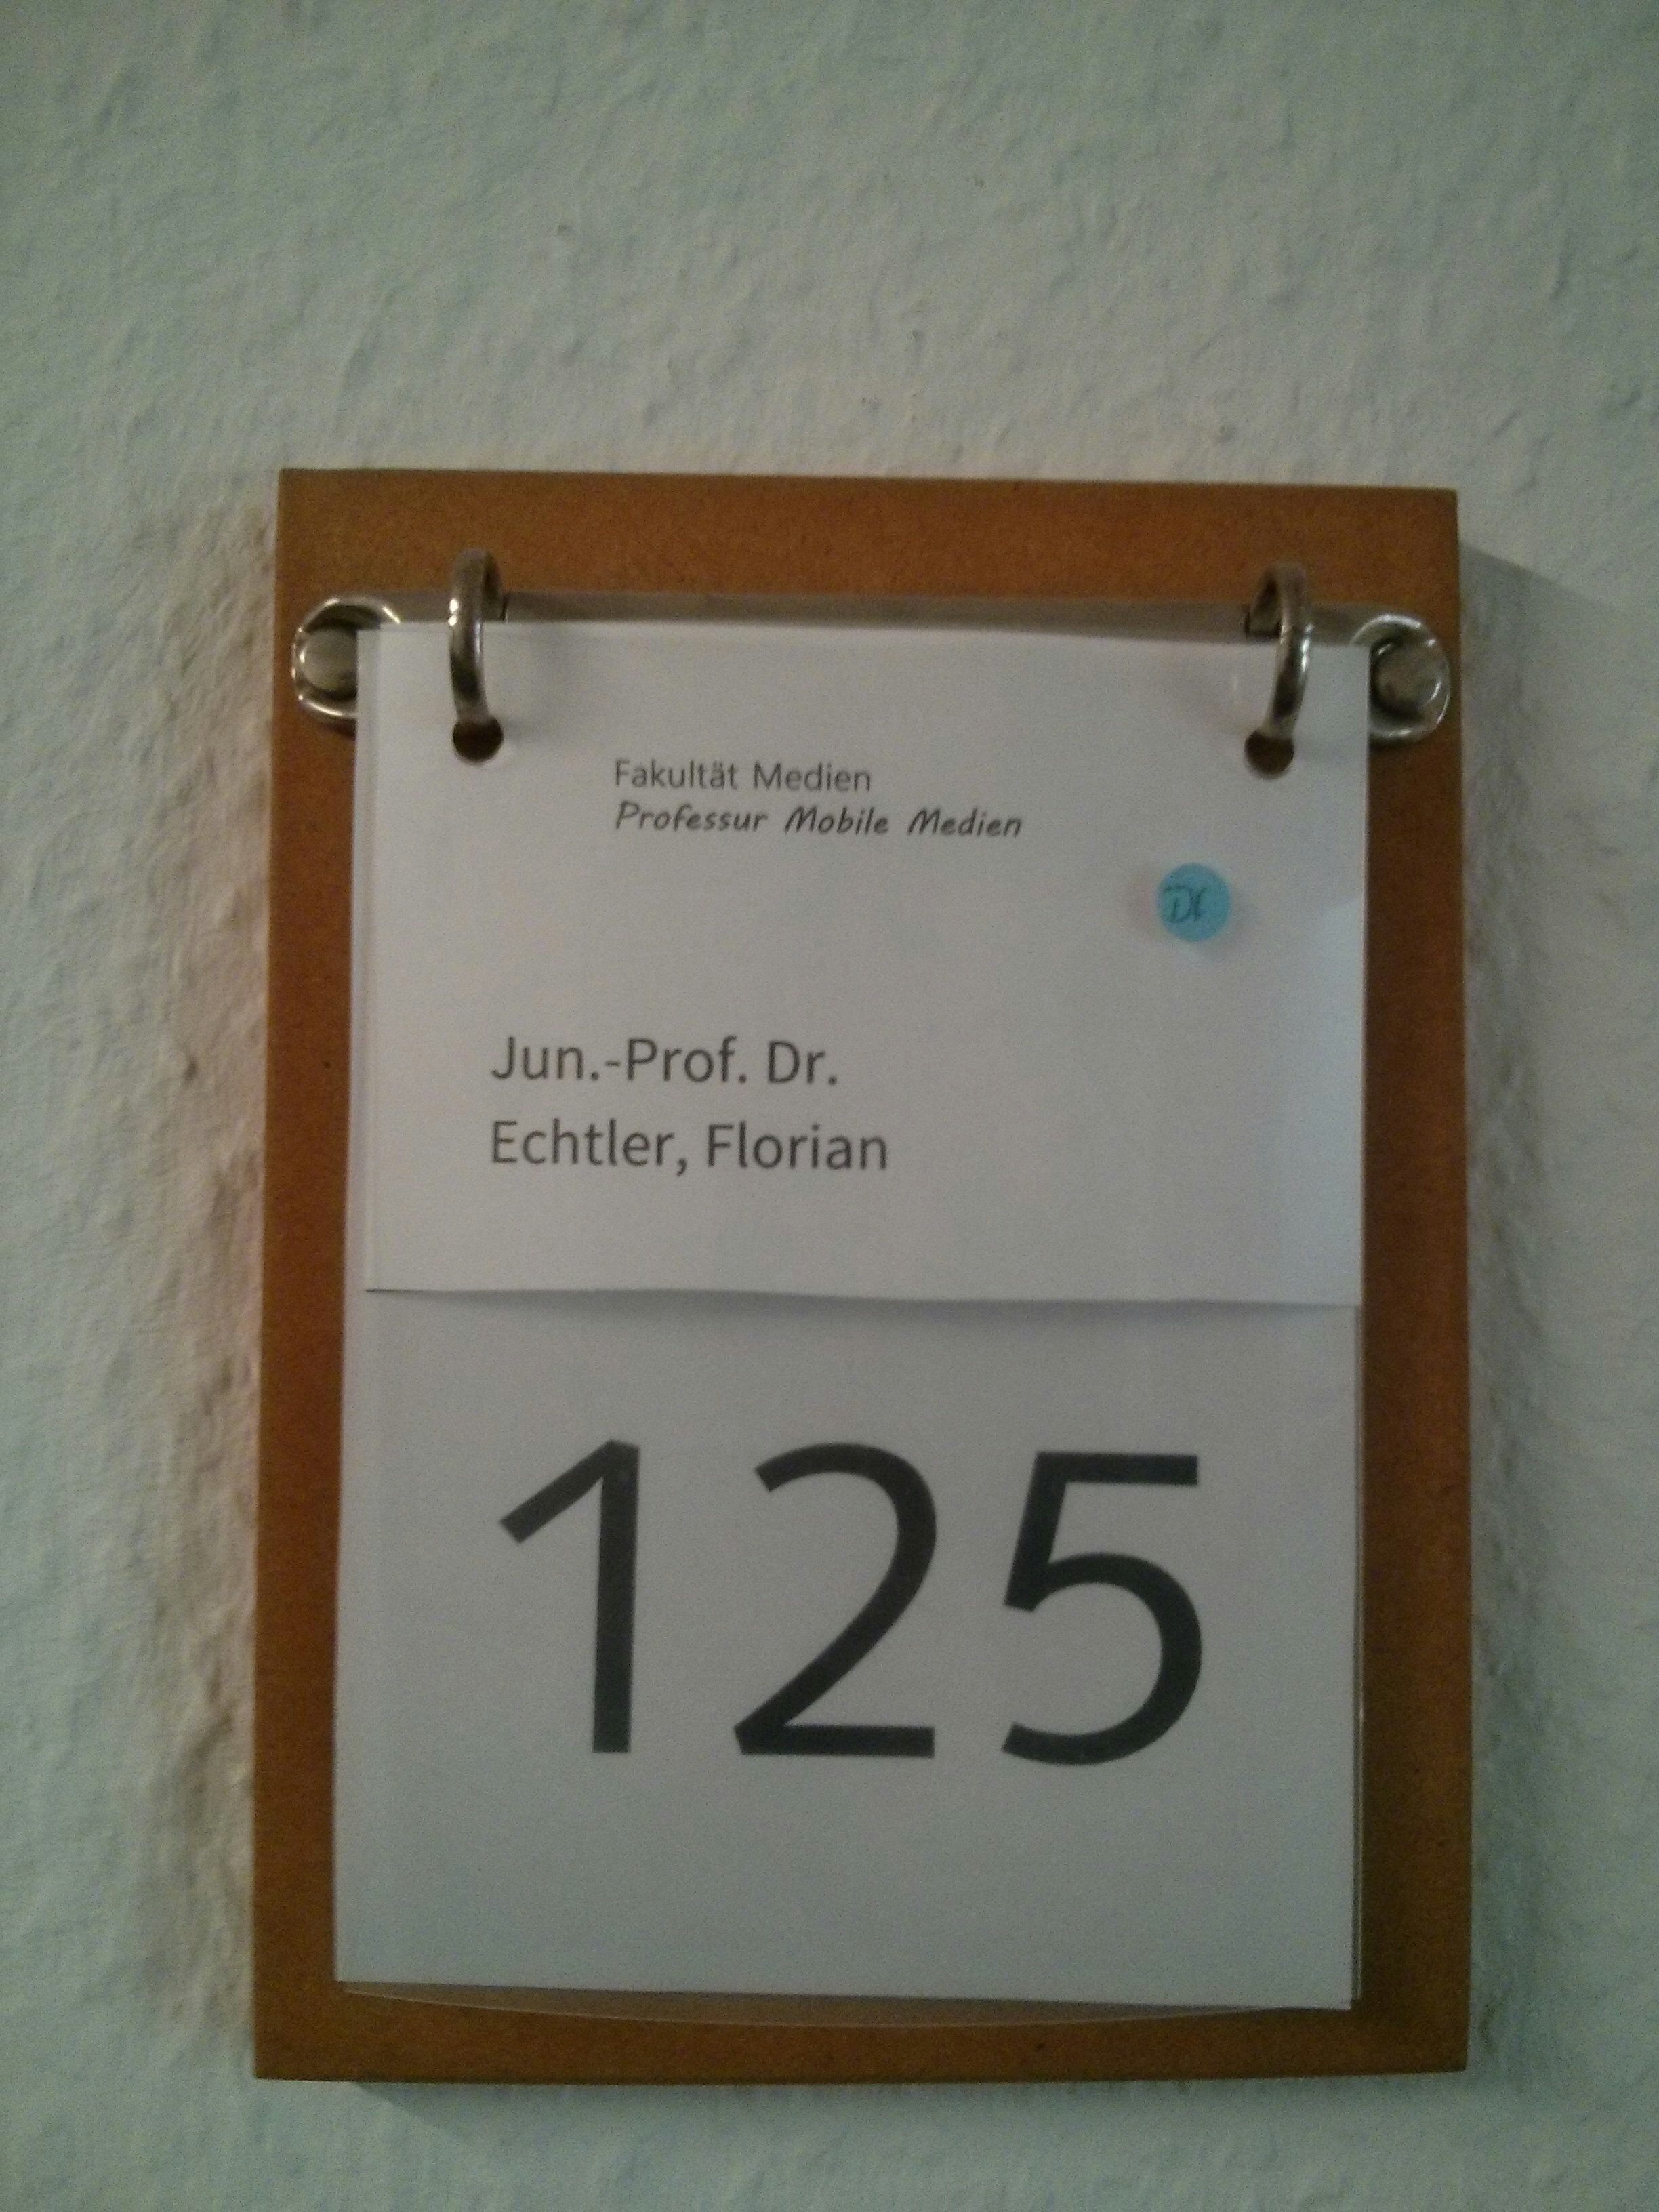
\includegraphics[width=0.5\textwidth]{./img/Tuerschild.jpg}
  \caption{Ein typisches Türschild in der Medienfakultät}
  \label{img:tuerschild}
\end{figure}\\
Dadurch, da sich die Rückwand des Tablets abschrauben ließ konnte ich zwei Löcher hinein bohren. Diese dienten zur Anbringung eines Drahtes, welcher über das Türschild gehangen werden konnte. Für dieses Experiment war die Aufhängung vollkommen ausreichend.\\
Für die Stromversorgung wurde das Ladekabel des Tablets verlängert, damit es an eine Steckdose im Büro angeschlossen werden konnte.\\
Als Testnutzer für das Experiment konnte ich zwei Mitarbeiter der Professur für Webtechnologien und Informationssysteme organisieren.
Diese Nutzer teilten sich ein Büro, wodurch nur ein Anzeigegerät benötigt wurde. Nach einer Einweisung zur Benutzung des Systems wurde klar, dass die zwei Tester nicht damit einverstanden waren, dass durch die Interaktivität des Boards jeder vorbeigehende Gast den dargestellten Inhalt nach belieben ändern konnte. Es hätte sein können, da durch die Anonymität der Gäste, das Board missbraucht werden könnte, um unangebrachte Skizzen zu zeichnen.
% Hier Beispiel mit Mensa Kinderhacksteak anstelle Rinderhacksteak
Aus diesem Grund habe ich für die Nutzer zwei verschiedene Ansichten erstellt:
\begin{itemize}
  \item Eine Backend-Sicht, auf der die Tester ihre Änderungen machen konnten.
  \item Eine Frontend-Sicht, die auf dem Tablet angezeigt wurde, nach 5 Minuten den aktuellen Stand abspeicherte und die Sicht auf den aktuellsten Stand der Backend-Sicht setzte.
\end{itemize}
\begin{figure}[h!]
  \centering
    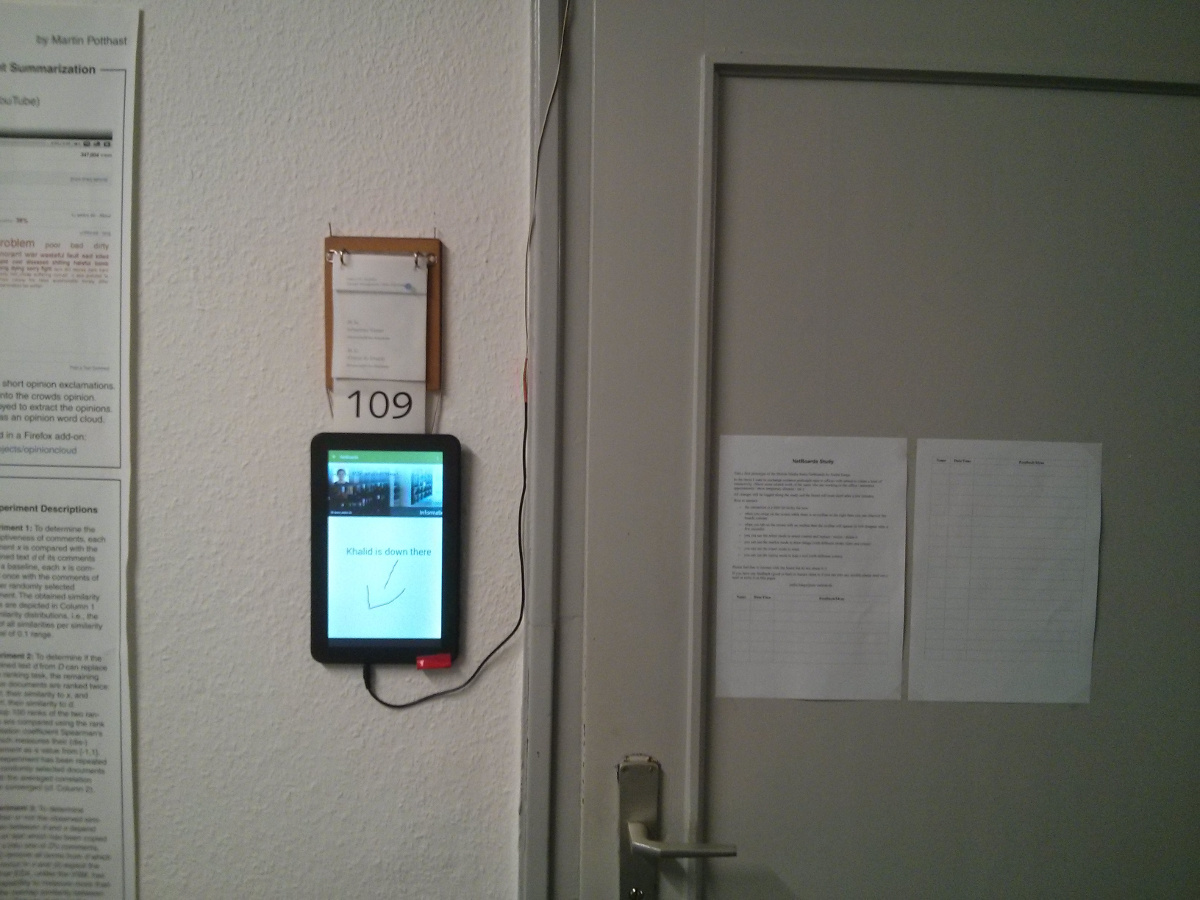
\includegraphics[width=0.7\textwidth]{./img/experiment01.jpg}
  \caption{Versuchsaufbau des Experiments}
  \label{img:experiment01}
\end{figure}



% Experiment Dauer
% 28.05.2015 - 08.06.2015
% 12 Tage
\section{Auswertung}\label{Auswertung}
Das Experiment lief 12 Tage. Die Nutzer erstellten sich zu Beginn einen Nutzeraccount und richteten ihr Board ein. Jeder der beiden lud ein Profilbild hoch und gab seinen Namen, sowie seinen akademischen Grad an.
Einer der Tester benutzte das Display um das Banner der Professur zu präsentieren (Abb. \ref{img:experiment02}) und um Gäste beispielsweise darüber zu informieren, dass er sich zur Zeit im Büro befindet (Abb. \ref{img:experiment03}).\\
Sehr erfreudig war, dass das Board viel Aufmerksamkeit zu erzeugen schien. Viele vorbeigehende Nutzer blieben stehen, um sich das Display genauer anzusehen und interagierten sogar damit. Dadurch entstanden viele Zeichnungen, wovon viele keinen tieferen Sinn hatten wie Beispielsweise die Zeichnung in Abb. \ref{img:experiment04}. Jedoch gab es auch ab und an Nachrichten, die direkt an die Besitzer des Boards gerichtet waren, wie das Bild einer Kaffeetasse mit einem Fragezeichen aus Abb. \ref{img:experiment05}, was die Frage nach einer Kaffeepause darstellen sollte.
\begin{figure}[h!]
  \centering
    \subfigure[erste Änderung der Nutzer]{
      \frame{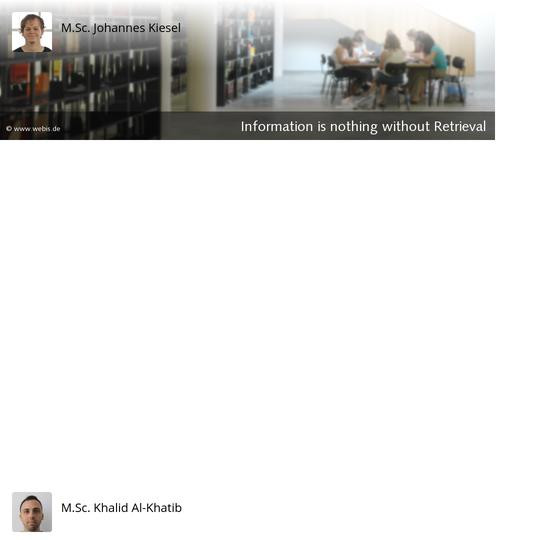
\includegraphics[width=0.4\textwidth]{./img/experiment02_empty.jpg}}
      \label{img:experiment02}
    }
    \subfigure[Statusangabe eines Nutzers]{
      \frame{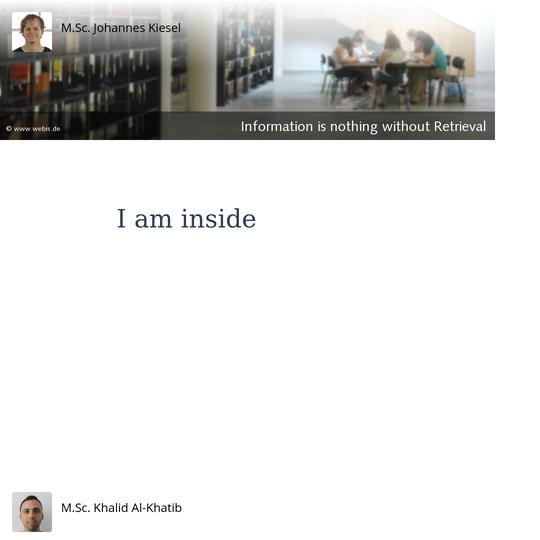
\includegraphics[width=0.4\textwidth]{./img/experiment03_statusContent.jpg}}
      \label{img:experiment03}
    }
    \subfigure[gezeichnetes Bild eines Gastes]{
      \frame{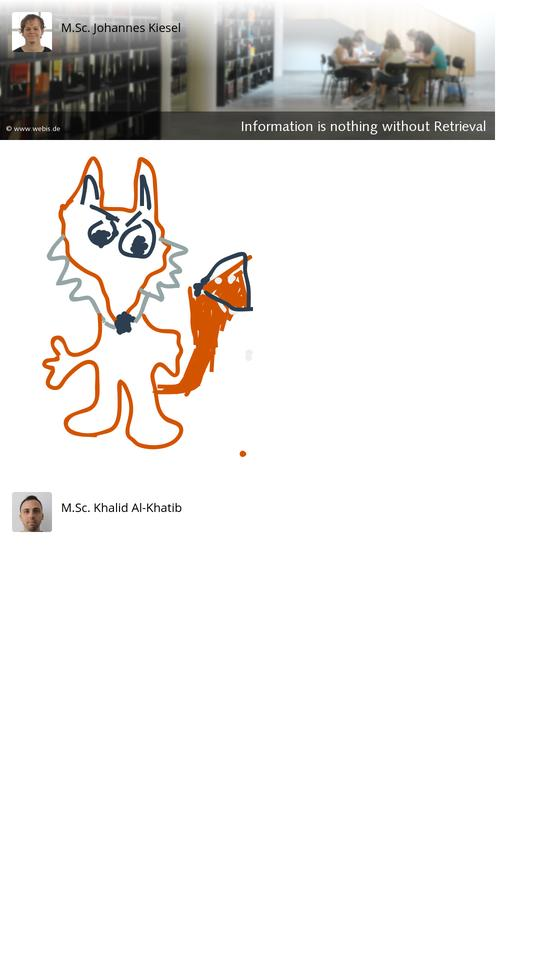
\includegraphics[width=0.4\textwidth]{./img/experiment04_fox.jpg}}
      \label{img:experiment04}
    }
    \subfigure[Frage eines Gastes]{
      \frame{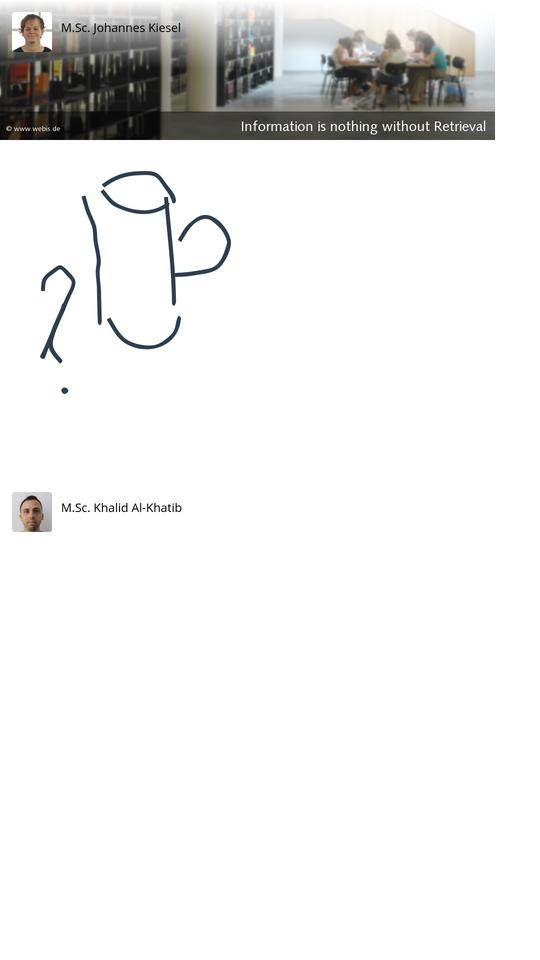
\includegraphics[width=0.4\textwidth]{./img/experiment05_coffee.jpg}}
      \label{img:experiment05}
    }
  \caption{Einige Beispielbilder}
\end{figure}
\\
\\
Nach Beendigung des Experiments führte ich ein Gespräch mit den Testnutzern, sowie mit einigen Gästen.\\
Es stellte sich dabei heraus, dass durch die geringe Auflösung des Tablets den meisten Benutzern gar nicht klar wurde, dass zwei Nutzer auf dem Board angemeldet waren. Man musste manuell in der Ansicht scrollen, um den Inhalt des zweiten Nutzers einsehen zu können. Jedoch war auch das ein Problem, da Scrolling nur möglich war, wenn die Sidebar ausgeblendet war. Die meisten Nutzer interagierten demnach nur mit der oberen Hälfte des eigentlichen Inhalts.\\
Ein weiteres Problem war, dass das Tablet eine sehr geringe Leistung hatte und das Touch-Interface nicht sehr genau war. Dadurch waren Interaktionen mit dem Board sehr langsam und ruckelig.\\
Positive Äußerungen gab es bezüglich angezeigter Statusmeldungen wie beispielsweise ``I am inside''. Die meisten Besucher fanden diese Meldung hilfreich, da sie deshalb wussten, ob der Mitarbeiter zur Zeit im Raum ist.
Weil zum Empfangen einer Benachrichtigung eine Browser-App erforderlich war, was den Testern nicht bewusst war, hatten sie keine Möglichkeiten darüber benachrichtigt zu werden, wenn jemand etwas auf ihrem Board änderte. Es wäre besser gewesen, wenn die Besitzer einfach eine Email erhalten hätten, wenn ihnen jemand etwas mitteilen wollte.
\\
\\
Als Schlussfolgerung des Experimentes entschied ich mich dazu ein eigenes System zu entwerfen.
Dieses System sollte gut auf Tablets laufen und für eine kleinere Bildschirmgröße angepasst sein. Dies erforderte, dass jeder Nutzer eine eigene Sicht bekommen sollte, da ansonsten auf dem Tablet zu wenig Platz wäre. Außerdem sollte es weniger als interaktives Whiteboard zu benutzen sein und mehr die Funktion von digitalen Pinnwänden übernehmen. Dadurch sollten nur noch die Besitzer die Möglichkeit haben den Angezeigten Inhalt zu ändern. Den Besuchern sollte dennoch möglich sein, mit den Besitzern in Kontakt zu treten, welche darauf eine Benachrichtiguns-Email erhalten sollten.
\chapter{BauhausBoards}\label{BauhausBoards}
Das neue Projekt bekam den Namen ``BauhausBoards''.
In einer Entwurfsphase entschied ich, wie das System aussehen und welche Funktionen es bieten sollte. Dabei flossen die Ergebnisse der Vorstudie und anderer Projekte mit ein.
\\
Als Voraussetzung sollten als Anzeigegeräte für die Türschilder weiterhin Tablets genutzt werden.
Der Entwurf wurde darauf in ein Programm umgesetzt, wobei manche geplante Funktionen geändert, entfernt oder neue hinzugefügt wurden. An manchen Stellen der Umsetzung kam es auch zu Problemen, die es zu lösen galt.
% - Ergebnisse der Vorstudie sollten enbezogen werden
% - sollte weiterhin auf Tablets als Anzeigegerät laufen
% - das was im Entwurf geplant wurde musste umgesetzt werden
% - dadurch entstanden Features
% - Während der Umsetzung traten diverse Probleme auf










\section{Entwurf}\label{Entwurf}
\subsection{Systementwurf}\label{Systementwurf}
Die Planung des Systems begann damit, die Plattform des Systems auszuwählen. Es gab die Möglichkeit eine Android-Applikation zu erstellen, die auf jedem Tablet installiert werden müsste. Dabei gäb es jedoch das Problem, dass die Nutzer auch von unterwegs mit der Anwendung interagieren sollten, wofür ein eigenständiger Server für die Datenverwaltung notwendig gewesen wäre. Außerdem müsste durch die unterschiedlichen Tablet- und Smartphone-Betriebssysteme neben Android, wie Apple IOS oder Windows Mobile, die App für jede Architektur portiert werden.
\\
Deswegen fiel die Wahl auf eine Web-Applikation. Zum Einen, weil jedes Tablet, jedes Smartphone und jeder PC Webseiten darstellen kann und es nicht nötig ist, extra eine App auf den Geräten zu installieren.
\\ \todotext{darauf eingehen, dass NetBoards auch eine Web-Applikation benutzt hat?}\\
%Zudem setzte das NetBoards Projekt ebenfalls auf eine Web-Applikation
Ein zentraler Webserver generiert eine Webseite mit allen nötigen Frontend Funktionen, die von allen Geräten mit Web-Browser (Clients) angezeigt werden kann. Dadurch sollte sich der Programmieraufwand auf Server- und Client-Funktionen einschränken.
\\
Die Applikation sollte nicht bei jeder kleinsten Interaktion mit der Webseite diese neu laden müssen. Das hätte einen viel zu großen Overhead erzeugt, da bei jeder Kommunikation statische Daten übertragen worden wären.
Deswegen musste der Server nur beim ersten Aufruf das Grundgerüst der Webseite mit allen Client-Funktionen ausliefern. Ein Teil der Funktionen würde dann Daten nachladen oder an den Server schicken, wodurch ein dynamischer Inhalt erzeugt wird.
Dies sollte mit dem ``CRUD'' (Create, Read, Update and Delete) Prinzip realisiert werden.
Der Server wartet, nachdem er eine Seite ausgeliefert hat, auf spezifische Anfragen des Clients und liefert dementsprechend Daten aus (Read) oder ändert den Zustand der Daten (Create, Update und Delete). Zudem gewährleistet dieses Prinzip, dass bei Verbindungsabbrüchen die Seite auf dem Client weiter läuft und nur so lange keine Daten ändern oder nachladen kann, bis die Verbindung wieder aufgebaut wurde.
\\
Die anfallenden Daten des Systems mussten in irgend einer Form auf dem Server gespeichert werden. Die beste Methode dafür war die Nutzung einer Datenbank. Anders als bei NetBoards, wo alle Daten als JSON\footnote{\quelle{JSON ist ein, für Menschen leicht zu lesendes und Maschinen leicht zu parsendes, Datenaustauschformat}{json:website}}-Dateien auf dem Server gespeichert wurden, sah ich diese Methode als geeigneter an. Mit einer Datenbank war es möglich Relationen besser darzustellen, Konsistenz zu bewahren und Redundanz zu vermeiden. Zudem sind damit Daten zentralisiert zusammengefasst, wodurch eine bessere Suche nach bestimmten Daten möglich ist.
\\
Die Wahl des Datenbanksystems fiel auf ``SQLite''\cite{sqlite:website}, da es das am meisten verbreitete relationale Datenbanksystem der Welt ist. Es war einfach zu benutzen und hatte eine gute Dokumentation.
\\
Das Gerüst der Webseite sollte auf HTML basieren, wobei die hauptsächlichen Client-Funktionen üblicherweise in Javascript umgesetzt werden. Da die Clients viele Funktionen bieten sollten und der Server nur zum Ausliefern der Webseite und für den Datenaustausch dienen sollte, machte es Sinn für den Server ``Node.js'' zu verwenden. \quelle{Node.js ist serverseitiges Javascript basierend auf Google Chrome's V8 Javascript Engine}{nodejs:website}.
\\
\\
In der Abb. \ref{img:Systemaufbau} ist der Aufbau des Systems zusammengefasst. Auf dem Server befinden sich der Webserver und die Datenbank. Der Webserver stellt Anfragen an die Datenbank und erhält dafür entsprechende Ergebnisse zurückgeliefert.
\\
Wenn ein Client die Adresse des Servers aufruft generiert der Webserver die Webseite und sendet sie mit allen benötigten Funktionen an den Client. Solange die Seite nicht explizit neu geladen werden soll, kommuniziert der Client danach nur durch CRUD Interaktionen mit dem Server.
\\
\begin{figure}[h!]
  \centering
    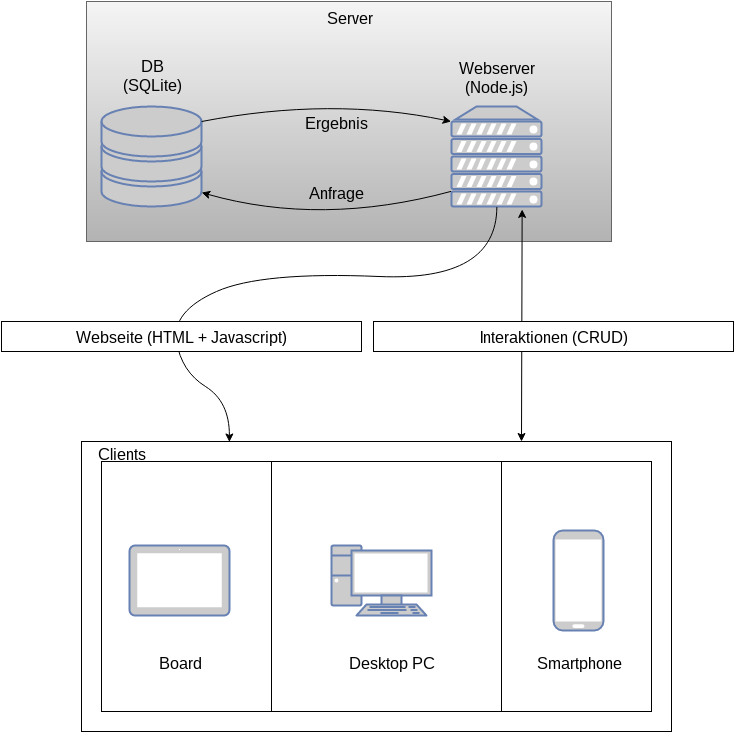
\includegraphics[width=0.8\textwidth]{./img/Systemaufbau.png}
  \caption{Bauhausboards - Systemaufbau}
  \label{img:Systemaufbau}
\end{figure}
\\
Da die Nutzer die Möglichkeit bekommen sollten, individuellen Inhalt präsentieren zu können, musste ein geeigneter Editor programmiert werden.
Damit sollte es möglich sein, einfache Zeichnungen anzufertigen, Texte zu schreiben oder Bilder hochladen zu können.
Es war wichtig, dass der Editor die Funktionen eines Whiteboards in manchen Zügen übernehmen oder möglicherweise sogar verbessern konnte.
\\
Folgende Whiteboard-Funktionen musste der Editor daher abbilden:
\begin{itemize}
  \item Zeichnen mit verschiedenfarbigen Stiften
  \item Entfernen von Zeichnungen mit einem Schwamm
  \item Anbringung von Bildern oder Ausdrücken per Magnet
  \item Neuanordnung von aufgehängten Elementen
\end{itemize}
Als Grundlage für den Editor entschied ich mich für die Javascript Bibliothek ``Paper.js''\cite{paperjs:website}.
Es ist ein Open Source Framework für die Darstellung und Manipulation von Vektorgrafiken, welches auch die Grundlage des Editors aus dem NetBoards Projekt bildete\cite{wood:2014}.
\\
\\
Eine weitere wichtige Entscheidung war, dass nur die an den Boards registrierten Nutzer den dargestellten Inhalt ändern können sollten, da sich in der Vorstudie herausstellte, dass durch die Anonymität der Besucher es häufig zu unerwünschten Änderungen kam.
Dadurch sollte ein weiterer Sicherheitsaspekt geschaffen werden, da keine andere Person die Daten ändern kann außer derjenige, der sie erstellt hat.
\\
Den Besuchern sollte jedoch weiterhin die Möglichkeit geboten werden mit den registrierten Nutzern in Kontakt treten zu können. Dies konnte mit einer separaten Nachrichtenfunktion realisiert werden.











\subsection{Interface-Entwurf}\label{Interface-Entwurf}
\subsubsection{Hauptansicht}\label{Hauptansicht}
Da den Gästen in der Vorstudie nicht bewusst war, dass mehrere Personen auf dem Board registriert waren, was der Größe des Tablets zu verschulden war, musste der vorhandene Platz anders aufgeteilt werden. Das NetBoards System teilte den Bereich verschiedener Benutzer räumlich, indem es den verfügbaren Platz durch die Anzahl der registrierten Benutzer teilte.
Auf einem 10,1 Zoll großem Tablet macht dieser Ansatz jedoch wenig Sinn, da bei mehr als einem Benutzer der verfügbare Platz zu klein wäre\abb{img:aufteilungMainView}.
\begin{figure}[h!]
  \centering
    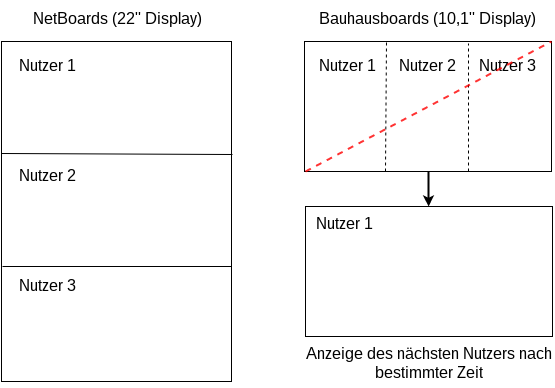
\includegraphics[width=0.68\textwidth]{./img/AufteilungMainView.png}
  \caption{Vergleich der Platzverteilung NetBoards - Bauhausboards}
  \label{img:aufteilungMainView}
\end{figure}
\\
Deswegen sollte jeder registrierte Nutzer die ganze Fläche zu Verfügung haben, wobei nach einer festgelegten Zeit die Sicht wechselt und die Daten des nächsten Nutzers anzeigt.
\\
Die Datenansicht sollte in zwei Schichten aufgeteilt werden. Zum einen eine Editor-Schicht für selbst gezeichnete Skizzen, Texte, Bilder und animierte Gifs, sowie eine Hintergrundschicht, in der die Nutzer eine Webseite anzeigen lassen können. Da NetBoards diese Funktion bereits bot und die Testnutzer in der Vorstudie diese ebenfalls nutzten entschied ich mich sie ebenfalls umzusetzen.
\\
Um auf der Webseite navigieren zu können musste es dafür ein Menü geben, die auf den Tablets nicht viel Platz wegnahm. Die beste Variante dafür war ein Sidebar, der standardmäßig eingeklappt war und sich per Klick oder Swipe-Geste öffnen ließ.
In diesem Menü sollten alle Navigationselemente zu untergebracht sein. 
\\
Um Informationen über die Nutzer anzeigen zu können wurde eine zusätzliche Fläche benötigt. Dafür sollte im oberen Bereich des Displays ein Teil nur für solche Informationen reserviert sein. In diesem Header konnte man das Profilbild, den Namen und eine Beschreibung des aktuell ausgewählten Nutzers darstellen.
In der Vorstudie wurde es sehr gut aufgenommen, dass einer der Nutzer seinen aktuellen Status angegeben hat. Deswegen sollte diese Funktion neben den Nutzerinformationen im Header zu finden sein.
\begin{figure}[h!]
  \centering
    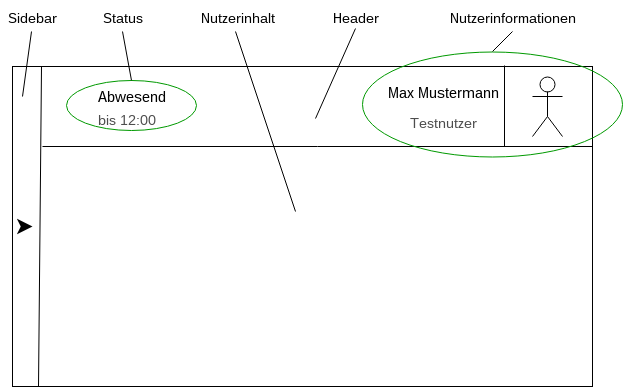
\includegraphics[width=0.7\textwidth]{./img/MainViewAufbau.png}
  \caption{Aufbau der Hauptansicht}
  \label{img:mainView}
\end{figure}
\\
%Messages
Damit die Gäste mit den Besitzern in Kontakt treten können musste es eine Nachrichtenfunktion geben. Dabei sollten die Benutzer, die eine Nachricht erstellen wollen, einen oder mehrere Besitzer auswählen können. Wenn sie das getan haben, soll der Editor aktiviert werden und die Besucher können eine Zeichnung oder einen Text zeichnen. Die Besitzer müssen, nachdem die Nachricht abgeschickt wurde, darüber informiert werden, dass jemand ihnen etwas geschrieben hat.
% - QR-Code, um mit Smartphone einzuscannen -> möglichkeit per smartphone Nachrichten zu hinterlassen

\subsubsection{Benutzer-Backend}\label{Benutzer-Backend}
Die Besitzer der Boards sollten ihren öffentlichen Inhalt ändern, einen Status setzten und empfangene Nachrichten lesen können.
Dafür müssen sie sich vorher im Benutzer-Backend authentisieren.
\\
Das Backend soll den Nutzern die Möglichkeit bieten, ihre Nutzerdaten, wie das Profilbild, die Benutzerbeschreibung oder das Passwort ändern zu können.
\\
Um die angezeigten Daten der Hauptseite anzupassen, wird der selbe Editor verwendet, der auch bei der Erstellung von Besuchernachrichten zum Einsatz kommt.
\\
Für den Status sollen die Nutzer einen kurzen Text und den Endzeitpunkt festlegen, der dann auf der Hauptseite angezeigt wird.
\\
Außerdem mussten sie die Möglichkeit bekommen, erhaltenen Nachrichten einsehen zu können. Ungelesene Nachrichten sollten dabei besonders gekennzeichnet sein.\\
Die Änderung der Benutzerdaten sollten in einem gesonderten Einstellungsbereich möglich sein.
\\
Da das Benutzer-Backend auch vom aufgehängtem Display aus erreichbar sein soll, damit die Nutzer beim verlassen des Raumes schnell einen Status setzen können, mussten sie sich schnell authentisieren können. Deswegen entschied ich mich für zwei Authentisierungsmethoden. Ein vierstelliger Pin sollte zur schnellen Anmeldung in das Backend dienen. Die Benutzereinstellungen konnten dann nach einer klassischen Passwortauthentisierung vorgenommen werden.

\begin{figure}[h!]
  \centering
    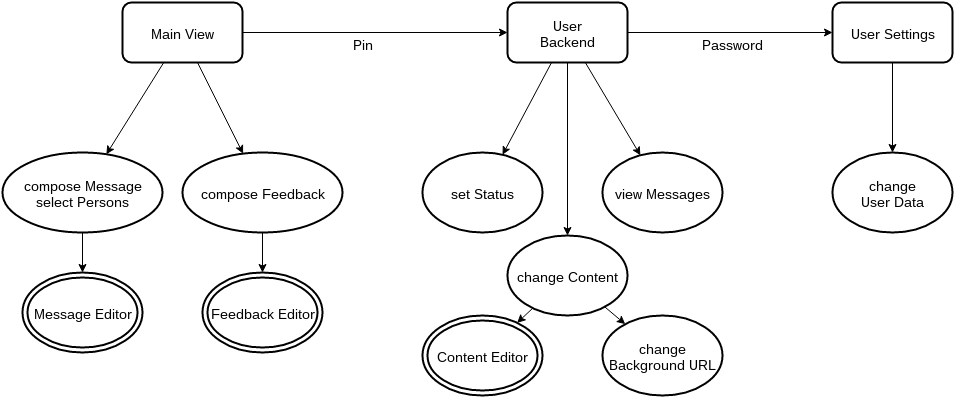
\includegraphics[width=0.9\textwidth]{./img/LocationsFrontend.png}
  \caption{Bauhausboards - Interface Funktionen}
  \label{img:Interface}
\end{figure}

\subsubsection{Administrator-Backend}\label{Administrator-Backend}
Der Administrator der Boards muss die Funktionen bekommen, das System verwalten zu können. Das beinhaltet das erstellen, ändern und entfernen von Nutzern, sowie Board-Instanzen.
\\
Zudem soll er für Studienzwecke die Inhalte und Nachrichten der Benutzer einsehen können.b

\subsection{Datenbankentwurf}\label{Datenbankentwurf}
Durch die geplanten Funktionen mussten anfallende Daten in einer Datenbank gespeichert werden.
Es bestand die Möglichkeit eine dokumentenbasierte oder eine relationale Datenbank dafür zu nutzen.
Eine dokumentenbasierte Datenbank hätte den Vorteil gehabt, dass alle Anfragen eine JSON-Zeichenkette zurückgeben. JSON wird häufig in der Verbindung mit Javascript und dessen Serverkommunikation verwendet.
Relationale Datenbanken hingegen verwenden eine Tabellenstruktur für die Speicherung von Daten. Mit ihnen lassen sich Beziehungen zwischen den Daten einfacher darstellen.
\\
Für die Datenbank von Bauhausboards entschied ich mich für eine relationale Datenbank, da die Einarbeitungszeit, um mit dokumentenbasierten Datenbanken umgehen zu können, zu lang gedauert hätte.
\begin{figure}[h!]
  \centering
    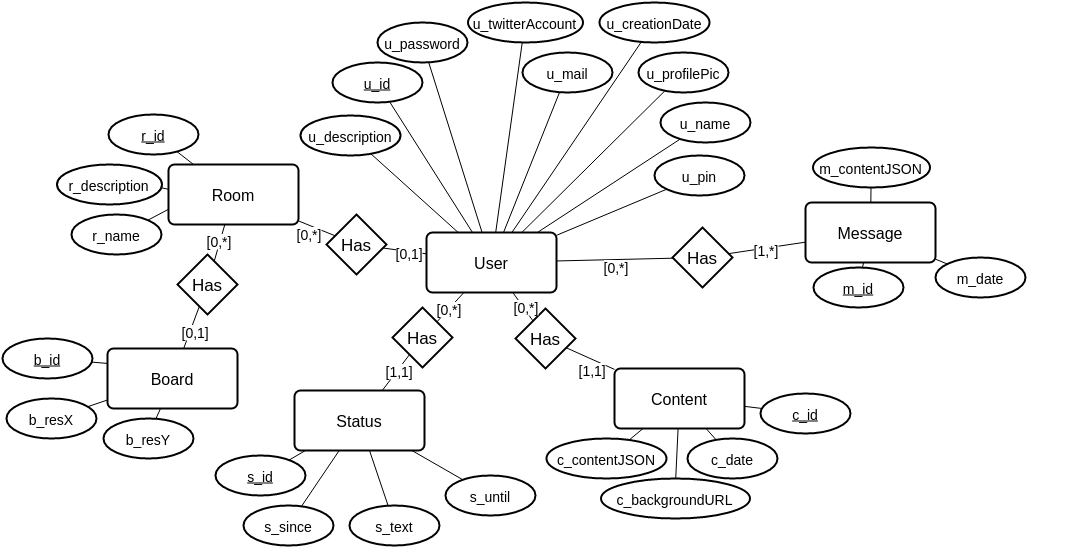
\includegraphics[width=0.75\textwidth]{./img/ER01.png}
  \caption{Bauhausboards - Entity Relationship Diagramm}
  \label{img:ER01}
\end{figure}
\\
Der Datenbankentwurf beinhaltete 6 Objektklassen, dargestellt als Tabellen. Um alle Objekte eindeutig beschreiben zu können wurde in jeder Tabelle eine ID als Primärschlüssel\footnote{Ein Primärschlüssel ist ein Attribut zur eindeutigen Identifikation eines Datensatzes} hinzugefügt.
\\\todotext{soll ich bei den Attributen noch auf die Datentypen eingehen?}\\
\subsubsection{User Tabelle}\label{User Tabelle}
Die User-Tabelle ist die Haupttabelle und dient zur Speicherung von Nutzeraccounts. Ein Nutzer muss auf jeden Fall einen Namen, eine Emailadresse, ein Passwort und einen Pin haben.
Zusätzlich können die Nutzer auch ein Profilbild, eine eigene Beschreibung und, wenn erwünscht, ein Twitter-Account angegeben werden.
Wenn ein Benutzeraccount erstellt wird, soll das aktuelle Datum mitgespeichert werden.
\\
Ein Benutzer kann entweder in einem oder keinem Raum arbeiten. Er kann beliebig viele Status und Inhalte erzeugen und beliebig viele Nachrichten erhalten.
\subsubsection{Board Tabelle}\label{Board Tabelle}
Diese Tabelle ist die digitale Repräsentation von tatsächlich aufgehängten Displays. Da verschiedene Tablets eine unterschiedliche Auflösung haben können, musste diese in der Datenbank für jedes Board gespeichert werden. Ein Board kann entweder noch keinem oder genau einem Raum zugeordnet sein.
\subsubsection{Room Tabelle}\label{Room Tabelle}
In dieser Tabelle werden die möglichen Räume, vor denen Boards aufgehangen werden können registriert. Jeder Raum hat einen Namen und möglicherweise eine Beschreibung. Ein Raum kann entweder keinem oder mehreren Boards zugeordnet sein. Zudem können beliebig viele Personen in einem Raum arbeiten.
\subsubsection{Content Tabelle}\label{Content Tabelle}
Mit dieser Tabelle werden die Inhalte von den Nutzern gespeichert. Ein Inhalt besteht aus einem JSON-Objekt und einem Erstelldatum. Wenn für den Inhalt eine Hintergrundwebseite angegeben wurde, wird deren Adresse ebenfalls an dieser Stelle eingetragen. Jeder Inhalt hat genau einen Nutzer, der ihn erstellt hat.
\subsubsection{Status Tabelle}\label{Status Tabelle}
Die Status Tabelle dient zur Speicherung von Nutzerstatus. Jeder Nutzerstatus hat einen Statustext, ein Erstelldatum, einen Endzeitpunkt und genau einen Ersteller. 
\subsubsection{Message Tabelle}\label{Message Tabelle}
In der Message Tabelle werden Nachrichten abgelegt, die von Besuchern erstellt wurden. Eine Nachricht hat einen Nachrichteninhalt und ein Erstelldatum. Da die Nachricht an mehrere Besitzer adressiert sein kann, hat jede mindestens einen Empfänger.
\\
\\
Die Relationen zwischen User und Message, sowie zwischen User und Room müssen jeweils über eine dritte Tabelle dargestellt werden. In diesen Tabellen werden dann nur die Primärschlüssel der beiden beteiligten Objekte gespeichert.






















\section{Umsetzung}\label{Umsetzung}
\subsection{Funktionen}\label{Funktionen}
\todotext{vll ein treffenderer name als Funktionen? vllt Bibliotheken?}\\
% Ich muss hier nicht auf jede kleine lib eingehen -> nur auf die wichtigsten
% hier kommt eine Überleitung vom Entwurf hin
Nachdem das der Aufbau des Systems geplant war, mussten diese Pläne in ein lauffähiges Programm umgesetzt werden.
Um die Entwicklung mit Node.js zu vereinfachen wurde das Framework Express\cite{express:website} verwendet. Damit ließ sich eine einfache Webapplikation erstellen.
\\
Da die hauptsächlichen Funktionen auf den Clients ausgeführt werden sollten, mussten diese in Javascript geschrieben werden.
Am wichtigsten war, dass die Seite sich nicht neu lud, wenn man durch sie navigierte. Dies wurde mit jQuery\cite{jquery:website} realisiert. jQuery ist eine Bibliothek zur einfachen Manipulation der HTML-Struktur einer Webseite. Mit ihr war es einfach, die dargestellte Ansicht anzupassen.
\\
Der Kern der Clientfunktionen war der Editor zum Erzeugen von Nutzer-Inhalten und Besuchernachrichten. Da Paper.js nur ein Framework war, musste das Interface dafür von Grund auf implementiert werden.
Voraussetzungen für Paper.js war, dass die Webseite für dem neuesten HTML5 Standard entwickelt wurde, da diese Version ein neues Canvas-Element bot, mit dem Grafiken gezeichnet werden konnten.
\\
Falls an einer Stelle der Seite Daten vom Server benötigt wurden oder Daten auf dem Server geändert werden mussten, wurde dies mit Ajax-Anfragen durchgeführt. Ajax (Asynchronous Javascript and XML) ist eine Funktion für asynchronen Datenaustausch zwischen einem Client und einem Server.
Während ein Client auf die Ajax-Antwort des Servers wartet können weiterhin andere Funktionen ausgeführt werden.
\\
% jquery touchswipe -> swipe tool für die swipe geste
Um die Sidebar auf Tablets leichter öffnen zu können nutzte ich TouchSwipe\cite{touchswipe:website}. Mit dieser Bibliothek konnten Swipe-Gesten zum aufruf von Funktionen genutzt werden.
\\
% cryptoJS hash lib für passwort hashes
Die Passwörter und Pins durften nicht im Klartext gespeichert werden.
Dafür wurde die crypto-js\cite{cryptojs:website} Bibliothek verwendet, um die sicherheitsrelevanten Daten mit SHA256\footnote{SHA256 (Secure Hash Algorithm 256) ist eine Krypto-Hashfunktion} zu hashen.
\\
% emailJS = mail tool
Damit die Besitzer der Boards benachrichtigt werden, wenn Gäste ihnen Nachrichten hinterlassen, musste der Server Emails verschicken können.
Die Bibliothek emailjs\cite{emailjs:website} brachte diese Funktion mit. Zusätzlich benötigte der Server zum Verschicken einer Mail einen eigenen Mailserver oder wenigstens einen Account an einem anderen Mailserver.
In den Benachrichtigungsmails sollte ein Link mit einem Token\footnote{Ein Token ist ein Attribut zur Freigabe von Daten zwischen Parteien(Wer den Token hat, kann die Datei lesen)} zu der jeweiligen erhaltenen Nachricht im System sein. Der Token wurde mit crypto-js beim Abspeichern der Nachricht auf dem Server erzeugt. Wenn der Empfänger auf den Link klickt, wird der Token geprüft und die Entsprechende Nachricht angezeigt ohne, dass sich der dieser authentisieren muss.
\\
Die Farbgestaltung der Seite wurde schlicht gehalten und orientierte sich an den Hausfarben der Medienfakultät der BUW.\\\todotext{mehr zur css gestaltung?}
\\
\\
Während der Umsetzung änderte sich die Entscheidung, alle Funktionen in einer einzigen Seite anzubieten, vom geplanten Konzept.\\
Im Konzept war ursprünglich geplant, dass der Administrator normal über die Seite die Administratorfunktionen ausführen kann. Da diese Funktionen aber rein funktional waren und nicht auf den Boards gebraucht wurden, ergab es mehr Sinn diese gesondert in eine zusätzlichen Webseite auszulagern.

% Editor Features
%Drag and Drop Images - URL wird geholt und ein neues Image wird erzeugt
%Pen
%text
%Stroke Size
%Color
%farbe von pen und text elementen ändern
%Auswahlwerkzeug:
%selektierung von einzelnen Objekten
%selektierung von mehreren objekten mit bounding box
%Popup
%löschen von markierten elementen
%Layering
%Kopieren
%Translation der Objekte in Bounding Box
%Scale der Objekte in Bounding Box
%Rotation der Objekte in der Bounding box
%Eraser Tool
%UNDO/REDO
%Gif Layer Support

% Background Feature (einfach nur eine hintergrundlayer ohne pointer events)

%caching of content for disconnects
%status set
%N/A marking of user image
% - Zudem sollen sie die möglichkeit bekommen sich als nicht anwesend markieren zu können, damit Gäste, die auf die Boards schauen schnell sehen, wer da ist und wer nicht

%Twitter API für den letzten Tweet eines bestimmten Nutzers 
% - Nutzer im Raum, die gern Twitter benutzen sollen die öglichkeit bekommen ihren TwitterAccount anzugeben, damit ihr letzter tweet auf ihrer Pinnwand angezeigt werden kann






\subsection{Features}\label{Features}
\todotext{das kann zu Funktionen, daher ist das Kapitel überflüssig}
% Unterschied zu Hermes / NetBoards
% jeder user hat eigene Pinnwand weil tablet resolution nicht so groß und dadurch wenig platz, mach keinen sinn für alle nutzer im raum nur eine pinnwand zu bieten (vergleich NetBoards) - switch betweeen them
% größeres Display als bei Hermes, kleineres als bei NetBoards
% Ähnlicher Editor auf selber Basis wie bei NetBoards
% Nutzer bekommen Mails, wie bei Hermes??

%background layer wie bei NetBoards

%nachrichten schreiben >> mail versenden mit unique token >> nachricht content direkt lesen mittels token
%  * nachricht an 1, 1+ oder alle im raum schicken
%  * direkte nachrichten gab es nur bei Hermes, bei NetBoards konnte man nur die Pinnwand direkt manipulieren
% feedback: hat einfach nur den editor















\subsection{Probleme}\label{Probleme}
Die Probleme, auf die ich während der Arbeit gekommen bin\\
%Editor:\\
%- Gif Layer Hack\\
%- Scale Problem\\
%- Stroke Size Problem\\
%Problem: Desktop Version dimensions
%- die Auflösung auf dem Desktop ist größer als auf dem Tablet
%- content, der auf dem Desktop weiter rechts/weiter unten erstellt wird, verschwindet auf dem tablet :(
%- Lösungsansätze:
%  # Canvas resize auf größeren Auflösungen
%  # anzeige von linien, wie es auf dem tablet angezeigt wird
%Problem Header
%- durch horizontale ausrichtung der tablets ist der Platz des header zu groß und wird verschwendet
%- wenn nur userimage, username, status, description usw angezeigt werden muss
%- Lösung: absolutes header div, welches oben rechts in der ecke ist
%  # content hat dadurch tatsächlich die größe des tablets
%  # platz wird nicht so stark verschwendet
%  # "toter winkel" oben rechts in den raw datas der images
%- die ganze css datei muss angepasst werden, da positionen und größen relativ zum header gesetzt waren
%- random server deadlock --> restart script
%- Message Email mit image direkt in der NAchricht im HTML als <img> element ging nicht, da  cross origin resource sharing(CORS) nicht aktiviert ist (origin-clean flag false) deswegen geht die Funktion .toDataURL("image/png") nicht
%   * Zudem ist es schwer in der mail ein paperJS project in ein canvas einzubinden
%   * deswegen die Überlegung beim erstellen der message das canvas objekt direkt zu exportieren

% gif:
% canvas element konnte nativ keine gifs anzeigen
%  -> lösung: gif layer
% wenn mehrere gifs des gleichen names: nur ein gif wird ausgeführt, die anderen sind statisch
\chapter{Studie}\label{Studie}
Um das System in der Praxis zu testen, musste im Anschluss eine Nutzerstudie durchgeführt werden.
Dies beinhaltete die Planung und Durchführung der Studie, sowie die Auswertung der Ergebnisse.
Es mussten die Rahmenbedingungen der Studie geplant und Testpersonen angeworben werden, die darauf in einem Interview Fragen beantworten und einen standardisierten Fragebogen zur allgemeinen Benutzung ausfüllen mussten.

\section{Entwurf}\label{Entwurf}
Nachdem die Umsetzung des Bauhausboards Systems abgeschlossen war, galt es einen Test mit Mitarbeitern der Medienfakultät der BUW durchzuführen.
\\
Dafür wurde am internen Rechenzentrum der Uni ein Linux Server mit 2,53GHz Intel Xeon Dualcore, 2GB RAM und Ubuntu Version 14.04 aufgesetzt.
Auf dem Server liefen Node.js, damit Bauhausboards ausgeführt werden konnte und Postfix\footurl{http://www.postfix.org} als Mailserver.
Dieser Mailserver konnte nur Emails an Adressen innerhalb des Universitätsnetzes verschicken, was für die Studie jedoch kein Problem darstellte.
\\
Als Displays wurden neue Tablets angeschafft, die mehr Leistung besaßen, als das Tablet aus der Vorstudie.
Es handelte sich dabei um vier Blaupunkt Discovery 1000c mit 10,1 Zoll Display, 1,33GHz AllWinner A33 Quadcore, 1GB RAM und Android\todotext{4.4 oder 5}. Mit vier Tablets konnten für die Studie vier Räume mit Displays ausgestattet werden.
\\
Damit die Benutzer, wie in der Vorstudie, nicht mit den vorinstallierten Applikationen der Tablets interagieren konnten, musste auch auf den neuen Tablets eine Kiosk-Applikation\footurl{http://www.android-kiosk.com} installiert werden.
\\
Zusätzlich zum Kiosk wurde eine Tasker-App\footurl{http://tasker.dinglisch.net} installiert.
Damit konnte man Aufgaben nach bestimmten Systemereignissen ausführen lassen.
Es wurde Task erstellt, der beim Start des Android-Systems automatisch die Kiosk-App startete, falls das System neu bootete.
\\
Als Diebstahlsicherung konnte man auf den Tablets Google Locate aktivieren.
Es diente zur Ortung der Geräte, falls diese gestohlen worden wären.
\\
\\
Um die Displays aufhängen zu können, musste eine geeignete Befestigungsmöglichkeit gefunden werden.
Jedoch sollten keine neuen Löcher zur Aufhängung an den Wänden neben den Büros entstehen.
Deswegen mussten die Displays erneut mit Hilfe der bereits aufgehängten Türschilder befestigt werden.
Da bei dieser Studie die Tablets nicht, wie in der Vorstudie, durch Löcher in der Tablet-Rückwand, angebracht werden konnten, musste die Befestigung anders ausfallen.
Zu diesem Zweck wurden 3D gedruckte Eckstücke \abb{img:Eckstuecke}, mit denen die Tablets befestigt werden konnten, auf eine Plexiglasplatte geschraubt \abb{img:fertigeAufhaengung}.
Diese Aufhängung nutzte die Bohrlöcher für die bereits vorhandenen Türschilder mit, wodurch keinerlei Eingriff in die Bausubstanz entstand.
\\\todotext{Bild von den Eckstücken und von der fertigen Aufhängung}\\
\begin{figure}%[h!]
  \centering
    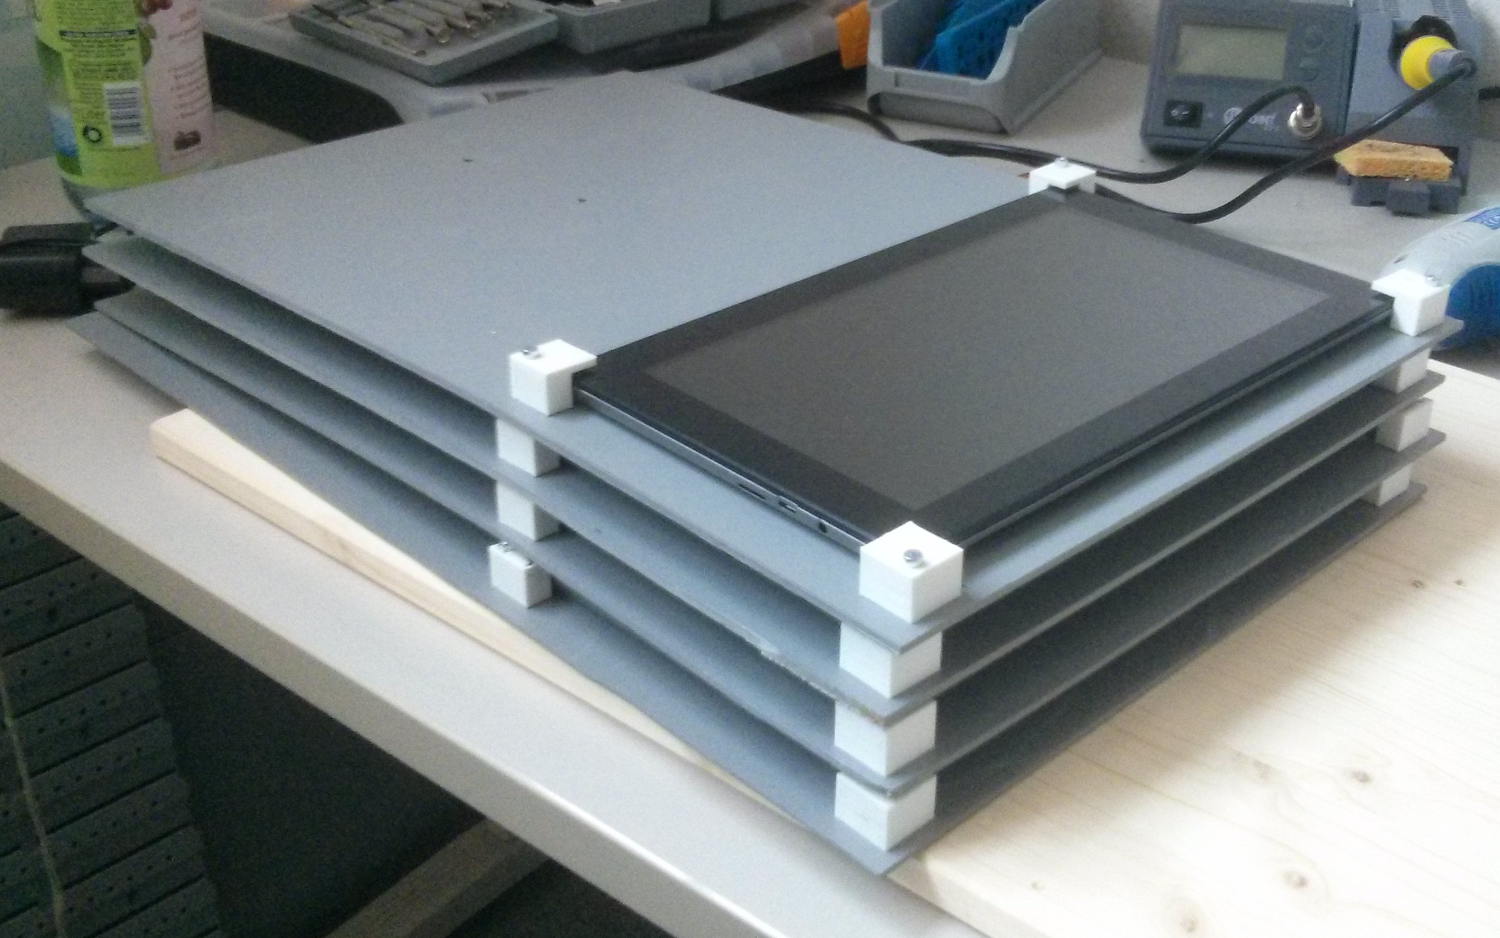
\includegraphics[width=0.85\textwidth]{./img/fertigeAufhaengung.png}
  \caption{Bauhausboards - Aufhängung}
  \label{img:fertigeAufhaengung}
\end{figure}
\\
Damit sich die Testnutzer mit der grundlegenden Funktion von Bauhausboards vertraut machen konnten, habe ich ein Benutzerhandbuch erstellt \todotext{in den ANhang oder so}.

% Nachdem Umsetzung abgeschlossen war: Test mit echten Nutzern
% Server mit NodeJS und Postfix aufgesetzt
% - Programm auf Server in Uni eingerichtet -> Spezifikationen? oder wurde das schon vorher angegeben?
% - Mailserver installiert, damit Server mails verschicken konnte (nur uni-intern)
% 4 Tablets angeschafft (Durch 4 Tablets -> 4 Räume zum Testen möglich)
%- Blaupunkt Discovery 1000c
%   * 10,1"
%   * CPU: Quadcore @ 1,33GHz
%   * Android 5.1
%   * 1GB RAM
%   * 1024x600 Auflösung (~17:10)
% Alle Tablets mit Kiosk-Mode Browser bestückt
%- Kiosk Mode Browser App auf Tablets um beenden der Bauhausboards App zu verhindern
%- Tasker zum automatischen start des kiosk modes nach systemstart - falls schlaue leute denken, sie können damit den kiosk browser umschiffen
%- Google Locate um Position des Tablets zu bestimmen, im falle eines Diebstahls
%- Rahmen: 4 Tablets -> 4 Räume
%- Wandbefestigung
%  * 3D gedruckte Eckstücke mit Loch um Tablets zu halten + zu sichern
%  * Holz/Blech Rückwand >> plexiglas
%  * Nutzung des vorhandenen Türschildes
%  * Fotos und 3D Model
%- Nutzer Tutorial zur Nutzung des Tools entworfen




\section{Durchführung}\label{Durchführung}
Da nur vier Räume mit Tablets ausgestattet werden konnten, war es von Vorteil, mit den vorhandenen Mitteln möglichst viele Testnutzer organisieren zu können.
Mir war es möglich, einige Mitarbeiter der Professur für Systeme der virtuellen Realität (VR) und der Professur für grafische Datenverarbeitung (CG) zur Teilnahme an meiner Studie zu gewinnen.
\\
Im Fachbereich der virtuellen Realität gab es drei Büroräume.
Zwei davon mit jeweils drei und einer mit zwei Mitarbeitern.
An der Professur für grafische Datenverarbeitung gab es zwei Mitarbeiter, die sich einen Raum teilten.
Diese Räume befanden sich alle im selben Gang der Fakultät.
\\
Da ein Mitarbeiter der VR Professur durch seine Forschungsarbeit nicht in seinem Büro sein konnte, nahm er nicht an der Studie teil.
\\
Somit konnten insgesamt 9 \todotext{Doktoranden und wie heißen die fertigen Doktoranden?} Testnutzer gewonnen werden.
\\
\\
Bevor die Studie beginnen konnte, mussten die Boards angebracht werden.
\\\todotext{Bild von aufgehängten Boards}\\
Außerdem musste eine gute WLAN Verbindung für sie gewährleistet sein.
\\\todotext{Grundriss des Gangs mit Tablets + Accesspoint}\\
Nachdem die Boards angebracht waren, wurde für jeden Benutzer ein Account erstellt, die Boards eingerichtet und die Nutzer kurz eingewiesen.
\\
Die Dauer der Studie beschränkte sich leider nur auf zwei Wochen.
Es sollte mindestens ein Wochenende eingeplant sein, weil sich das Benutzerverhalten nach diesen zwei freien Tagen ändern konnte.
\\
Während der Studie kam es gelegentlich dazu, dass einige Testnutzern Fragen zu bestimmten Funktionen hatten, welche direkt geklärt wurden.
Das System wurde gut genutzt und einige Gäste hinterließen den Testern Nachrichten.



\section{Auswertung}\label{Auswertung}
Nach Abschluss der Studie sollten alle Teilnehmer Interviewt werden.
Dazu musste vorher ein Fragenkatalog erstellt werden, um von den Testnutzern Feedback zu den wichtigsten Funktionen des Systems zu erhalten.
\\\todotext{mehr}
\subsection{Interview}\label{Interviews}
%- Aufnahme des Interviews (Audiofile)
% 330min Interview = 5h30min
% Aufteilung in Nachrichten empfangen, Nachrichten schreiben, Statusmeldungen, Nutzerinhalte, Editor, Boardfunktionen, Allgemeines
\subsubsection{Nachrichten empfangen}\label{Nachrichten Empfangen}
% Nachrichten empfangen
%  - mit den Nutzern die empfangenen Nachrichten durchgegangen um Herauszufinden, wofür die Gäste die Funktion genutzt haben
%  - Größtenteils keine ernst gemeinten Nachrichten (Spaßnachrichten, ``temporäres Grafitty'')
%  - ab und an Fragen, ob man zusammen Mittag essen gehen will oder ob Nutzer zugegen ist

%  - es war in keiner Nachricht ersichtlich, wer deren Autor war
%  - wurde von den Meisten Testnutzern bemängelt, dass sie den Autor nicht identifizieren konnten (sie konnten nur ab und an vermuten, wer es war)

%  - Nutzer wurden gefragt, wie man ihnen sonst eine Nachricht hinterlassen konnten
%  - die meisten meinten: per mail
%  - aber auch: postIt, tel, klopfen, sms(dafür müssen aber kontaktdaten da sein), usw

%  - Nutzer gefragt, ob es für sie anders war, über das Board eine Nachricht zu erhalten
%  - war praktisch, ``Die Zeichnung macht es anders'' (also positiv, dass Zeichnungen drin waren) es schafft eine persönliche Note, aber für manche war es nicht anders als eine normale mail(und demnach gut)

% - Alle haben dadurch, da sie per mail benachrichtigt wurden, es direkt gelesen, da sie auch direkt auf den link in der mail klicken konnten und sich deswegen nicht extra anmelden mussten

% - einige Nutzer fanden es gut, dass man ihnen eine Nachricht hinterlassen konnten, wenn sie grade nicht im Büro waren
% - als größtes Manko empfanden die Testnutzer, dass sie nicht sehen konnten, wer die Nachricht geschrieben hat
% - andere fanden es zu umständlich, einen einfachen text einzugeben, da die Touchauflösung des Tablets zu gering war
% - außerdem wurde es gut aufgenommen, dass man für die KOmmunikation mit den Besitzern nicht extra ein eigenes Gerät brauchte, da die Boards vor den Büros hingen

% - Verbesserungsvorschläge: autorkennzeichnung, voicemail, videomail, Vordefinierte Nachrichtenkategorien(dem Anliegen entsprechend), Vereinfachung durch weniger untermenüs
%%%%%%%%%%%%%%%%%%%%%%%%%%%%%%%%%%%%%%%%%%%%%%%%%%%%%%%%%%%%%%%%%%%%%%%%%%%%%%%%
\subsubsection{Nachrichten schreiben}\label{Nachrichten schreiben}
% selber Nachrichten schreiben
% - Auf die Frage, ob die Testnutzer einem anderen Besitzer eine Nachricht auf ihr Board hinterlassen haben, meinten die meisten, dass sie selber nur die Besitzerrolle wahrgenommen hatten und keinem eine Nachricht hinterlassen haben
% - das hatte den Grund, da sich die meisten Tester persönlich sehr gut kannten und die meiste Kommunikation mündlich durchführten
% - Einem Nutzer war der ganze Nachrichtenprozess zu viel Aufwand (und es war ihm zu versteckt)
% - ein paar Testnutzer nutzen es, um einen anderen Nutzer zu fragen, ob er mit zum Mittagessen mitkommen wollte
%%%%%%%%%%%%%%%%%%%%%%%%%%%%%%%%%%%%%%%%%%%%%%%%%%%%%%%%%%%%%%%%%%%%%%%%%%%%%%%%
\subsubsection{Status}\label{Status}
% Statusfunktion
% - die meisten Testnutzer haben die Funktion direkt genutzt oder aber sich ihren Status auf ihre Pinnwand geschrieben
% - davon haben alle Nutzer bis auf einen die Funktion vom PC aus genutzt, der andere wollte es am Board ändern, war aber der meinung, dass es für ihn zu kompliziert war, den status zu ändern (der meinung waren auch einige andere Testnutzer)
% - übliche Statustexte waren: ``busy'' oder ``im DBL zu finden'' oder im Meeting oder ganz einfach N/A
% - wie gesagt einige fanden das system zu kompliziert, vorallem das Interface (es bot zu viel auf einmal und war zu schwer zu erreichen)
% - andere wiederum fanden es gut, dass es dieses feature gab und man gesondert seinen aktuellen status kennzeichnen konnte
% - nützlich für gäste, um zu wissen, wann der Besitzer wieder da ist
% - Kollegen von Testnutzern mussten nicht wegen dessen status behelligt werden 
% - die meisten Nutzer haben den Status vor dem Verlassen des Büros geändert, wenn sie essen gegangen sind oder ins Meeting
% - auf die Frage ob Vordefinierte Status sie eher dazu animieren würden, das Feature zu nutzen meinte die Mehrzahl, dass es das würde

% - Die Auswertung ergab, dass die N/A Funktion zum Ausgrauen des Nutzerbildes nicht gebraucht wird

% - viele meinten, dass der Status zu unoffensichtlich ist und besser gekennzeichnet werden müsste oder komplett heraus genommen werden sollte, da man das auch alles über den COntent machen könnte
% - Ein Nutzer meinte, er würde seinen Status nur von unterwegs ändern, wenn er dem system eine mail mit dem statustext schicken könnte oder es per app machen könnte
% - Die Funktion sollte komplett vom Board genommen werden und nur für die Desktop-Version zugägnlich sein

% - der grund warum einige das Feature nicht genutzt haben war, dass ``sie eh die ganze Zeit da waren und es deswegen nicht brauchten'' oder es nicht für nötig hielten, da eine geschlossene Tür schon statusindikator genug ist ``Wenn die Tür zu ist, bin ich nicht da''
%%%%%%%%%%%%%%%%%%%%%%%%%%%%%%%%%%%%%%%%%%%%%%%%%%%%%%%%%%%%%%%%%%%%%%%%%%%%%%%%
\subsubsection{Nutzerinhalt}\label{Nutzerinhalt}
% Content ändern
% - der Content wurde hauptsächlich für spaß benutzt, es wurden Bilder und gifs hochgeladen und präsentiert. Aber es wurde auch zum Teil zur präsentation von fachlichem Inhalt verwendet ``um von außen einen schnelleren Eindruck zu gewähren, was ich mache''
% - andere Nutzen diese Funktion wie schon gesagt zur ANzeige ihres Status

% - entweder wurde der Editorlayer oder aber der Backgroundlayer zur Anzeige von Bildern/Gifs genutzt weil es war für die NUtzer nicht offensichtlich, wie man im Editorlayer bilder hochlädt --> einbau eines buttons dafür
% - genutzt für Webseiten (Nachrichten oder Seite der Professur)
% - Backgroundlayer wurde größtenteils positiv aufgenommen, wäre aber besser als poweruserfunktion
% - ein Nutzer meinte: Nutzer sollten selber über Background-Interaktivität entscheiden können

% - alle Nutzer haben nicht das twitterfeature genutzt, da fast alle keinen twitteraccount hatten
% - der eine Nutzer, der einen acc hatte, würde das feature nicht nutzen, da er privaten inhalt sonst präsentieren müsste

% - NUtzer fanden es interessant, da technologie neu war, man bewegten Inhalt präsentieren konnte oder einfach nur aus spaß
% - die nutzer, die es nicht benutzten hatten entweder keine Zeit einen content zu erstellen oder ihnen ist nichts eingefallen

% - übliche änderungszeit war zur Mittagszeit in der pause
% - leider ist benutzung mit der zeit eingeschlafen (nur am anfang der studie, danach weniger genutzt)

% - schön war es, dass es ab und an auch gäste gab, die auf den content von besitzern eingegangen sind und ein gespräch deswegen entstanden ist

% - von den meisten wurde es positiv aufgenommen: der persönliche Aspekt ``Sehr gut war die Möglichkeit selber Kreativ zu werden''
% - auch gut war es, dass man damit INformationen präsentieren konnte
% - am besten fanden die TEster, dass man damit gifs anzeigen konnte

% - einige Benutzer fanden wieder die bedienung zu kompliziert und, dass es zu viele features gab, dass man es auch hätte vereinfachen können
% - zu viele schritte, bis content geändert wurde --> weniger klicks desto besser

% - es wäre wahrscheinlich ernster benutzt worden, wenn es ganz offiziell da hängen würde oder es kommuniziert worden wäre, für welchen Content es vorrangig genutzt werden sollte
%%%%%%%%%%%%%%%%%%%%%%%%%%%%%%%%%%%%%%%%%%%%%%%%%%%%%%%%%%%%%%%%%%%%%%%%%%%%%%%%
\subsubsection{Editor}\label{Editor}
% Editor Benutzung
% - fast alle (außer 2) haben den Editor benutzt
% - sie haben es dafür benutzt um bspw eigene Arbeit zu skizzieren, texte zu zeichnen oder einfach nur spaßzeichnungen zu machen
% - die anderen meinten die benutzung wäre zu versteckt im backend
% - da die icons nicht wie in den üblichen editoren waren, waren sie nicht eindeutig(color=underline,selector wie rectangleZeichnen,undo-redo->geschwungene pfeile)
% - einigen war nicht von anfang an bewusst, dass sie bilder und gifs per drag and drop einbinden können (sie benutzten dafür die hintergrundlayer) -> musste ihnen erst gezeigt werden   ---> lieber Hinweis auf Funktion machen + extra upload button
% - es war schlecht, dass es keine autoskallierung für bilder und keine vordefinierten formen gab
% - außerdem wurde es bemängelt, dass das ausgewählte werkeug zu wenig hervorgehoben wurde

% - positiv war, dass er recht intuitiv zu benutzen war, dass er postIt ähnlich war

% - ``Es war für den Rahmen in dem es lief ausreichend''
% - ein Nutzer meinte, dass das schon allein als Boardfeature reichen würde
% - ausmalfeature wäre noch gewünscht
% - wekzeuge sollten dauerhaft angezeigt werden
%%%%%%%%%%%%%%%%%%%%%%%%%%%%%%%%%%%%%%%%%%%%%%%%%%%%%%%%%%%%%%%%%%%%%%%%%%%%%%%%
\subsubsection{Boardfunktionen}\label{Boardfunktionen}
% Allgemeine Boardfunktionen
% - es war für einige Tstnutzer nicht ersichtlich, wo sie sich im backend befanden, ob sie noch angemeldet sind und wer überhaupt angemeldet ist
% - deswegen sollte lieber das BAckend vom Frontend getrennt werden und vereinfachen (da jetzt zu viele klicks notwendig waren)
% - Alle Nutzer waren der Meinung, dass 2 Authentisierungen übertrieben sind
% - wenn Frontend und Backend getrennt wären, bräcuhte man nur eine Authentisierungsmethode
% - ein Nutzer war sogar der Meinung Passwortauthentisierung komplett weg zu lassen ``auch wenn es Vandalismus Tür und Tor öffnet''

% Frage, was sie als Vor- und Nachteile gegenüber PostIts, Whiteboards und Pinnwänden sehen
% positiv:
% - digitaler/dynamischer content
% - produziert keinen müll
% - die Besitzer werden direkt über Nachrichten informiert(per mail)
% - privacy(nur empfänger kann nachricht lesen)
% - keiner kann Nachricht löschen - postIt/whiteboardnachrichten aber entfernbar
% - Erstellung von Content per Remote
% - Kontaktaufnahme, selbst wenn Kontaktdaten unbekannt oder man kein geeignetes device zur hand hat
% - macht spaß
% - daten werden archiviert

% negativ
% - kostet energie
% - teurer als postIts
% - wird nur als spielerei wahrgenommen + Statusmeldungen im endeffekt nur peripher von Gästen wahrgenommen (postIts werden ernster genommen)

% - Die Größe der Boards fanden alle angemessen und hätten nicht unbedingt größere Boards gebraucht

% - viele waren der Meinung, dass der Wechsel zwischen den Benutzern nervig war
% - sie hätten lieber gewollt, dass die Nutzer parallel angezeigt werden, sodass man dann direkt auf den Benutzer klicken könnte um ihn eine Nachricht zu schreiben
% - dadurch hat man auch eine direkte sicht darauf, wer alles im Raum arbeitet, wer davon grad nicht verfügbar ist und was so dessen Status ist
% - dafür wäre auch in Kauf genommen, dass nur 1/3 Platz für Content zu Verfügung steht


%%%%%%%%%%%%%%%%%%%%%%%%%%%%%%%%%%%%%%%%%%%%%%%%%%%%%%%%%%%%%%%%%%%%%%%%%%%%%%%%
\subsubsection{Allgemeine Anmerkungen}\label{Allgemeine Anmerkungen}
% Allgemeine Anmerkungen
% - Studie war zu kurz um sich wirklich dran zu gewöhnen, weswegen die Funktionalität nicht in den Arbeitsprozess mit eingegangen ist
% - Teilweise waren die Menüpunkte nicht eindeutig bezeichnet
% - ``es war schön, dass man darüber Nachrichten empfangen konnte''
% - Für einen Testnutzer war es zu viel Aufwand, wenn man etwas auswählen musste oder durch das menü navigieren musste ``Keiner möchte ewig vor seinem Büro stehen und da rum klicken'' --> deswegen Trennung Frontend/Backend
% - Am besten wäre für zusätzliche Funktionalität eine Poweruser Einstellung
% - ein Nutzer meinte die Boards sind gute Notleuchten und dass sie gute Blickfänger sind

% Sidebar:
% - viele fanden es nervig, dass die sidebar immer wieder zu ging
% --> lieber auf Desktop dauerhaft anzeigen
% - autoclose nervig im Editor ``Du sitzt am Schreibtisch, arbeitest und hast dir deine Werkzeuge hingelegt. Dann kommt ständig deine Freundin und räumt dein zeug weg.''

% Board:
% - Touch genauigkeit zu unpräzise
%%%%%%%%%%%%%%%%%%%%%%%%%%%%%%%%%%%%%%%%%%%%%%%%%%%%%%%%%%%%%%%%%%%%%%%%%%%%%%%%









% Ergebnisse der Interviews
%   * manche Nutzer haben nichtmal das Tutorial gelesen ...
%   * Großteil der Nutzer meinte, dass es unersichtlich ist, wer alles im Raum arbeite und es besser wäre, dass man auf den ersten Blick erkennen könnte, wer alles drin arbeitet (sowas wie Nutzerliste Rechts unter Header)
%   * Ein Bug wurde entdeckt, dass wenn man noch keinen Content eingestellt hatte und man dann einen Hintergrund setzen will man ausgeloggt wird, da eine exception geschmissen wurde (Lösung eigene Background Tabelle in der DB)


\subsection{UEQ Fragebogen}\label{UEQ Fragebogen}






% UEQ Fragebogen nach Testlauf
% was ist UEQ
% Ergebnisse des UEQ
\chapter{Ausblick}\label{Ausblick}
\section{Zusätzliche Features}\label{Zusätzliche Features}
Welche Features noch nützlich wären

%- Beakon Authentifizierung mit dem Tablet
%- Gruppen Nachrichten, für bspw gruppen von mitarbeitern in mehreren Räumen
%- gespeicherte Statustexte (die häfigsten statustexte als template anbieten)
%- Image direkt in der Email
%- Browser/Desktop Plugin
%- Touch Projector??
%- Key Support für Desktop



\section{Nutzung}\label{Nutzung}
Ziel: Nutzung in der ganzen Uni


%- es wäre schön, dass wenn das Tool in der ganzen uni genutzt wird
%- abwesenheits information
%- informationen über wichtige daten
%- auflockerung des Arbeitsumfelds
%- anregung zum nachfragen zu arbeiten
% Bibliography
%\bibliographystyle{plainnat} % requires package natbib. An alternative is apalike
\bibliographystyle{unsrt}
\bibliography{literature}    % load file literature.bib

\end{document}

